\chapter{深度学习的可学习性}
\label{chap:deep-learning-theory}

一个网络已经把样本中的邮件全部分对，继续增加参数以后，它在新邮件上的错误率却还可能下降。
这并不符合一种常见直觉：模型越复杂，越容易记住样本，也就越容易过拟合。困难在于，
“能够记住样本”只描述网络的表达能力，并没有说明训练算法最终选择了什么假设。
同一个网络架构既可以表示有用的分类函数，也可以表示只记住样本的函数。

前几章已经提供了两条分析途径。VC维和一致收敛考察整个假设空间，算法稳定性则考察
训练结果对样本变化的敏感程度。第~\ref{chap:convex-learning-and-stability}章进一步说明，
稳定性需要与经验最优性结合，才能得到可学习性保证。本章在神经网络中验证这些一般
条件：权重范数怎样限制函数复杂度，训练过程怎样选择解，以及样本变化怎样传递到
参数、预测和损失。

因此，参数大小、训练中的特征和参数分布并非彼此独立的泛化原因。它们只有通过
具体的复杂度、稳定性或期望风险推导，才能成为学习保证的一部分。
这些分析也需要保留网络表示目标关系的能力，避免为了获得较小的泛化上界而排除
期望风险较低的假设。对于Transformer和大语言模型，还需要区分文档抽样、
词元依赖、上下文学习和长度变化，才能明确所证明的泛化究竟指什么。

\section{神经网络的学习问题}
\label{sec:network-learning-problem}

\subsection{网络与学习目标}

前馈网络通过逐层变换把输入转换成预测分数。每一层先用权重矩阵组合上一层的数值，
再用激活函数逐坐标变换结果。例如，ReLU函数$\phi(a)=\max\{0,a\}$保留正数、
把负数置零，使多层模型不再等价于一个线性变换。暂时省略偏置项，$L$层网络写为
\begin{equation}
 f_{\bm W}(\bm x)=\bm W_L\phi\bigl(\bm W_{L-1}\phi(\cdots\phi(\bm W_1\bm x)\cdots)\bigr),
 \label{eq:feedforward-network}
\end{equation}
其中$\bm W_\ell\in\mathbb R^{d_\ell\times d_{\ell-1}}$，$d_0$是输入维度。
把全部可训练参数排列成向量$\bm\theta\in\mathbb R^p$，也可将网络记为$f_{\bm\theta}$。
参数量$p$说明需要存储多少个可调数值，深度$L$说明输入依次经过多少层变换。
它们都不直接等于假设空间的VC维。

给定独立同分布样本$S=(z_1,\ldots,z_n)\sim\mathcal P^n$，其中$z_i=(\bm x_i,y_i)$，
学习算法通过减小经验风险选择参数：
\[
 \hat R_S(\bm\theta)=\frac1n\sum_{i=1}^n\ell(f_{\bm\theta}(\bm x_i),y_i),
 \qquad
 R_{\mathcal P}(\bm\theta)=\mathbb E_{(\bm x,y)\sim\mathcal P}
 \ell(f_{\bm\theta}(\bm x),y).
\]
经验风险由已有样本计算，期望风险描述同一数据分布下的新样本表现。
本章在分布已明确时简写为$R(\bm\theta)$。损失函数会随问题变化，涉及分类错误率时
明确使用零一损失；涉及梯度下降的精确推导时则说明所用的平方损失或逻辑损失。

若存在参数使给定样本的经验风险为零，就称该模型能够在这份样本上\term{插值}
（interpolation）。平方损失下，插值要求每个预测数值都等于标签；零一损失下，
插值只要求每个类别预测正确。交叉熵则通常只能在分数不断增大时趋近零，不能把
“分类全部正确”与“交叉熵已经等于零”混为一谈。\term{过参数化}
（overparameterization）通常表示参数相对于样本或拟合约束十分充足；$p>n$是常用的
粗略指标，但能否插值还取决于架构、数据和损失。

\subsection{VC维与样本量}

早期研究把神经网络看作一个由架构限定的假设空间，再使用VC维分析所需样本量。
Baum与Haussler在1988年的工作中研究了网络规模与泛化所需样本数的关系，重点对象
包括阈值网络\scite{baum1988size} 这条途径继承了二分类理论：只要能控制架构所表示的
分类假设的VC维，就能得到分布无关的统计学习保证，而不必先解释训练算法的每一步更新。

网络的VC维不仅取决于参数量，也取决于计算结构。对于分段线性网络，
Bartlett等给出了接近紧致的结果：以$p$表示参数量、$L$表示层数，ReLU网络的VC维
具有$O(pL\log p)$量级的上界，并存在达到$\Omega(pL\log(p/L))$量级的架构，
其中下界在相应的参数范围内成立\scite{bartlett2019vc}
这里的下界是对某些架构的存在性结论，并不意味着每个具有$p$个参数的网络都达到该容量。

将这种容量估计代入二分类学习基本定理，就得到网络的统计可学习性结论。
下面把网络结构的分析与学习保证的推导分开，以免把“存在一个学习算法”误读为
“梯度下降一定能够找到所需参数”。

\begin{theorem}[有限VC维网络的不可知PAC样本量保证]
\label{thm:network-vc-pac}
设固定架构所表示的二分类假设空间为$\mathcal H$，其VC维为有限数$d\geq1$，
并满足前述可测性条件。对于零一损失，存在通用常数$c>0$，使得任意
$\varepsilon,\delta\in(0,1)$和任意分布$\mathcal P$下，只要
\[
 n\geq c\frac{d\log(2/\varepsilon)+\log(2/\delta)}{\varepsilon^2},
\]
每个经验风险最小化算法输出的$\hat h$都以至少$1-\delta$的概率满足
\[
 R_{\mathcal P}(\hat h)\leq\inf_{h\in\mathcal H}R_{\mathcal P}(h)+\varepsilon.
\]
\end{theorem}
\begin{proof}
由有限VC维的一致收敛结论，在所给样本量下，可以使事件
$\sup_{h\in\mathcal H}|\hat R_S(h)-R_{\mathcal P}(h)|\leq\varepsilon/2$
以至少$1-\delta$的概率成立。在该事件上，对任意$h\in\mathcal H$有
\[
 R_{\mathcal P}(\hat h)
 \leq\hat R_S(\hat h)+\frac\varepsilon2
 \leq\hat R_S(h)+\frac\varepsilon2
 \leq R_{\mathcal P}(h)+\varepsilon.
\]
对右侧的$h$取下确界即可。证明使用了ERM的经验风险比较性质，没有给出实现ERM的
计算方法。
\end{proof}

因此，固定有限架构的统计可学习性并不是一个悬而未决的问题。实际困难常发生在另一个
尺度：当前只有$n$个样本，而网络容量给出的充分样本量远大于$n$。此时定理仍然正确，
却可能只能给出大于1的零一损失下的期望风险上界，无法解释已经观察到的低错误率。
若算法只找到近似ERM，还需把经验风险的优化误差加入上界。

\subsection{过参数化的挑战}

现代深度学习把这个差距表现得十分突出。Zhang等关于随机标签的实验显示，
一些深度网络既能拟合真实标签，也能拟合随机打乱的标签\scite{zhang2021rethinking}
拟合随机标签说明架构的表达能力很强，但两种训练结果的期望风险可以相差很大。
容量理论考察假设空间允许的最坏情形，不能单凭架构容量区分这两种结果。
图~\ref{fig:learning-deep-selection}把这三个对象画在同一张图中：外层区域是架构能够表示的
全部假设，内层区域是把当前样本全部拟合正确的假设，实心点是算法最终选出的一个假设。
泛化分析需要解释这个点在新输入上的表现，不能只观察外层区域有多大。

\begin{figure}[!htb]
 \centering
 % 大容量假设空间、插值解集合与优化算法的选解偏差。
\begin{tikzpicture}[x=1mm,y=1mm,font=\footnotesize]
  \fill[FigureInput!7] (0,0) ellipse (49 and 32);
  \draw[FigureInput,thick] (0,0) ellipse (49 and 32);
  \node[font=\kaishu\scriptsize,text=FigureInput] at (0,27) {架构可表示的假设空间};

  \draw[FigureLoss,very thick]
    plot[smooth cycle,tension=0.8] coordinates {(-31,-7) (-15,10) (5,13) (28,4) (17,-14) (-8,-18)};
  \node[font=\kaishu\scriptsize,text=FigureLoss] at (-3,-23) {经验风险为零的插值解};

  \draw[BookMuted,dashed,->] (-45,25) .. controls (-31,19) and (-27,8) .. (-18,4);
  \draw[BookMuted,dashed,->] (-45,18) .. controls (-25,11) and (-12,5) .. (0,2);
  \draw[BookMuted,dashed,->] (-45,11) .. controls (-22,4) and (6,0) .. (17,-3);
  \fill[FigureModel] (0,2) circle (2.2);
  \node[font=\kaishu\scriptsize,text=FigureModel,align=left,anchor=west] at (5,16)
    {优化器、初始化与正则化\\共同选择的一个解};
  \draw[book arrow,FigureModel] (7,14) -- (1.5,4);

  \node[font=\kaishu\scriptsize,text=BookMuted,align=center,text width=95mm] at (0,-38)
    {容量描述整个假设空间；泛化还取决于算法选择了哪个假设。};
\end{tikzpicture}

 \caption{架构、样本和算法分别限定不同对象。架构决定能够表示的假设，样本确定哪些假设
 能够插值，初始化、优化算法和正则化共同决定最终输出。架构相同并不意味着算法选出的
 假设具有相同的期望风险。}
 \label{fig:learning-deep-selection}
\end{figure}

图中的内层区域可能同时包含两种完全不同的分类假设。一种只记住已经出现的邮件，
遇到新邮件便采用任意默认分类；另一种利用促销词、链接等特征之间的关系预测类别。
采用零一损失时，它们在当前样本上的经验风险都可以为零，后者却可能在新邮件上继续有效。
增加参数以后，这两种假设都可能更容易被表示出来，所以“能拟合样本的解更多”
本身并不能决定期望风险上升还是下降。

图中的箭头强调了算法的选择作用。即使架构和样本保持不变，初始化、步长、优化器或
正则化改变，也可能把算法带向不同的插值解。要解释实际网络的泛化，就需要寻找比
“这个网络有多少参数”更细的依据：哪些解具有较小的有效复杂度，训练又为什么偏向它们。
这也是后面分别研究参数大小、训练轨迹与参数分布的共同起点。

过参数化也不必然导致更严重的过拟合。某些模型的期望风险在接近插值阈值时上升，
越过该阈值后反而下降，形成\term{双重下降}（double descent）曲线\scite{belkin2019double} 图~\ref{fig:learning-double-descent}给出这种形态的定性示意。
接近插值阈值时，拟合标签中的噪声可能需要很敏感的解；参数进一步增加后，可供选择的
插值解更多，算法可能找到范数较小或对扰动较不敏感的解。第二次下降依赖数据分布和
选解方式，不能推成“增加参数总能降低期望风险”。

阅读图~\ref{fig:learning-double-descent}时，需要分别观察经验风险与期望风险。
虚线到达零附近，表示模型已经能够拟合当前样本，并没有说明样本之外的预测也正确。
实线在插值阈值附近的峰值，表示某些选解方式此时对数据扰动十分敏感；右侧的下降则说明，
继续增加参数以后，算法有可能选择更适合预测新输入的插值解。这三种现象的区别，
正是单独观察经验风险无法解释的部分。

例如，欠定线性回归可以有无穷多个插值解。从零初始化出发的梯度下降选择其中的
最小欧氏范数解，而不会等概率地选择任意一个解。增加参数可以改变这个最小范数解及其
对噪声的响应，也就可能改变期望风险。第~\ref{sec:implicit-bias}节将完整证明这种选解
现象；这里先保留一个结论：过参数化的作用必须连同算法一起分析。

\begin{figure}[!htb]
 \centering
 % Reproducible teaching construction; source and input record in figures/plots/volume1-risk-and-shift.py/.json.
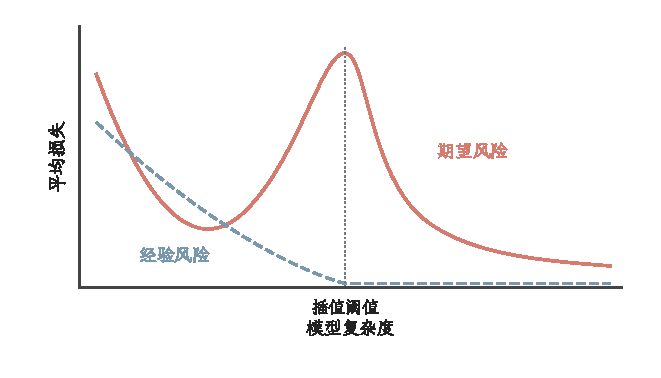
\includegraphics[width=\linewidth,trim=0 5mm 0 0,clip]{figures/plots/double-descent.pdf}

 \caption{双重下降的定性示意。虚线表示经验风险，实线表示一种可能出现的期望风险变化。
 图中曲线用于说明概念，不是实验数据，也不表示所有网络都出现第二次下降。}
 \label{fig:learning-double-descent}
\end{figure}

这些现象要求理论进一步说明算法选择了什么。范数界限制所选函数的大小与变化幅度；
初始参数梯度通过神经切线核确定近似固定的特征空间；梯度更新的动力学决定算法偏好的解；
参数分布则描述神经元群体的演化或训练结果附近的一组网络。这些研究在时间上相互交叠，
后来的方法也继续使用早期的复杂度与稳定性工具。

\subsection{从一般学习理论到神经网络}
\label{sec:deep-general-learning}

这些解释最终都要回答同一个问题：网络在样本上的损失已经较低时，怎样保证新样本上的
期望损失也低。第~\ref{chap:convex-learning-and-stability}章已经给出了分析框架。
对于输出属于比较空间$\mathcal H$的算法$A$，记
\[
 \begin{aligned}
 \Delta_n&=\mathbb E_S\bigl[R(A(S))-\hat R_S(A(S))\bigr],\\
 \rho_n&=\mathbb E_S\left[\hat R_S(A(S))-
                         \inf_{h\in\mathcal H}\hat R_S(h)\right].
 \end{aligned}
\]
在相关期望存在时，有
\begin{equation}
 \mathbb E_S R(A(S))-\inf_{h\in\mathcal H}R(h)
 \leq\Delta_n+\rho_n.
 \label{eq:deep-risk-decomposition}
\end{equation}
因为对于每个固定$h$都有$\mathbb E_S\hat R_S(h)=R(h)$，
所以$\mathbb E_S\inf_h\hat R_S(h)\leq\inf_h R(h)$，代入便得到该式。
其中$\Delta_n$是期望泛化差，$\rho_n$表示算法距离经验最优还有多远；
两者同时受控，才能获得相对于$\mathcal H$的低超额期望风险。
训练只降低经验风险，未必同时减小$\Delta_n$。

前章的一致收敛和算法稳定性给出了控制$\Delta_n$的两条途径。
前者同时控制一个函数空间中所有假设的经验风险与期望风险之差，后者利用算法实际输出
对样本变化的反应。二者考察的关系不同：VC维研究固定输入上的不同预测，稳定性
研究不同训练样本产生的输出。一个网络架构的假设空间不变，训练算法的稳定性却可能
随着初始化、正则化和优化方式而改变。

参数大小可以同时参与这两条途径。若预先限制权重范数，可以研究这个受限函数空间的
复杂度；若研究样本替换后的参数变化，权重范数又可能控制参数变化被放大为损失变化的
程度。后一种推导还需要证明相邻样本产生的参数确实接近，单独限制参数大小并不够。
参数分布也要通过分布距离或信息量进入期望风险分析，不能只凭训练结果具有某种
分布形式就认定泛化良好。

这些方法仍须遵守前面的不可学习性结论。对于零一损失、任意输入与标签联合分布下的
二分类PAC学习，无限VC维的假设空间不可学习，换用稳定性分析也不能改变这一结论。
后文不显含网络宽度的保证，会明确保留范数、分类间隔或数据分布等条件；
它们回答的是这些条件下的期望风险问题，并不自动给出整个无限VC维分类空间的
分布无关PAC保证。

以下各节会分别说明所控制的期望风险、样本量的作用和训练算法还需满足的条件。
其中，高概率期望风险界、对样本取平均的期望风险界和经验风险下降速度是不同的保证，
比较它们时必须保持损失函数与概率含义一致。

\section{基于参数大小的可学习性}
\label{sec:network-norm-bounds}

上一节遇到的困难是，同一个大网络既能拟合随机标签，也能学到可推广的关系。
按参数数量计算的VC维需要同时覆盖这两种行为，因此可能给出过大的样本量要求。
如果训练实际选出的假设只使用了假设空间中较受约束的一部分，就有理由改用这部分
假设的复杂度来估计期望风险。权重范数提供了一种可以计算的约束方式。

这里的“参数大小”指权重向量或矩阵的范数，不是参数个数。
直观上，模型为了分别迁就每个样本的偶然波动，可能需要很强的局部变化；
限制权重共同产生的放大能力，可以减少这类变化。
上一章的正则化也控制参数大小，但本节先从假设空间的复杂度出发，考察给定范数范围内
所有网络的经验风险与期望风险之间的关系，暂不要求解释参数是怎样训练出来的。

这种做法可以使泛化界不直接依赖网络宽度，却带来了新的问题。
多层网络中不同范数怎样组合，参数缩放会不会改变结论，分类间隔又应怎样计入，
都需要重新说明。即使这些问题解决了，较小的范数界也只评价所得假设，
不会自动保证梯度下降找到它。因此，本节先建立参数大小与期望风险的联系，
后面的理论再讨论训练过程如何产生这样的解。

\subsection{权重大小与分类间隔}

参数量相同的两个网络，可以对输入变化表现出完全不同的敏感程度。在线性预测中，
$|\langle\bm w,\bm x-\bm x'\rangle|\leq\|\bm w\|_2\|\bm x-\bm x'\|_2$，
权重范数直接控制输入扰动被放大的程度。网络范数界沿着这一思路，把约束从
“允许多少个参数”转向“这些参数共同表示多大的函数”。Bartlett在1996年的研究中
已经系统提出，适当条件下，权重大小可以比网络规模更直接地决定泛化保证\scite{bartlett1996weights}

分类还需要考虑预测分数离决策边界有多远。真实类别为第一类时，分数$(3,2,0)$和
$(2.01,2,0)$都给出正确分类，但前者领先第二名1分，后者只领先0.01分。
后一种预测更容易被小扰动改变。这种领先幅度称为分类间隔。

\begin{definition}[分类间隔]
\label{def:network-margin}
设$f_{\bm W}:X\to\mathbb R^K$是分类分数函数。
其在带标签输入$(\bm x,y)$处的分类间隔定义为
\begin{equation}
 \operatorname{margin}_{\bm W}(\bm x,y)
 =f_{\bm W}(\bm x)_y-\max_{j\neq y}f_{\bm W}(\bm x)_j.
 \label{eq:network-margin}
\end{equation}
对于取值为$\{-1,+1\}$的二分类标签和标量分数$f(\bm x)$，定义间隔为$yf(\bm x)$。
\end{definition}

正间隔表示正确类别的分数更高。若每个类别分数的变化不超过$\alpha$，多分类间隔的
变化不超过$2\alpha$，所以原间隔大于$2\alpha$时预测仍然正确。
范数与间隔需要一起使用：只把输出分数放大，既增大权重范数也增大间隔，
并没有改变分类函数或实际错误率。

\subsection{不显含宽度的期望风险界}

两层ReLU网络可以说明范数约束怎样替代直接的参数计数。隐藏层越宽，可用的特征
越多；如果输出权重的绝对值之和固定，网络就不能同时无限放大所有特征。
下面允许隐藏单元数任意大，但要求这一总量受到控制。

\begin{theorem}[两层网络的范数与期望风险]
\label{thm:two-layer-norm-risk}
在抽样前固定$A,B,r,\gamma>0$。设$\|\bm x\|_2\leq r$，并令
\[
 \mathcal F_{A,B}=\left\{\bm x\mapsto\sum_{j=1}^m a_j\phi(\bm w_j^\top\bm x):
 m\in\mathbb N,\ \sum_{j=1}^m|a_j|\leq A,\ \|\bm w_j\|_2\leq B\right\},
\]
其中$\phi$为ReLU函数。则任意输入样本上的经验Rademacher复杂度满足
\[
 \widehat{\mathfrak R}_S(\mathcal F_{A,B})\leq\frac{2ABr}{\sqrt n}.
\]
对于独立同分布的二分类样本，标签取$\{-1,+1\}$，以至少$1-\delta$的概率，
所有$f\in\mathcal F_{A,B}$同时满足
\begin{equation}
 \mathbb P_{(\bm x,y)\sim\mathcal P}\{yf(\bm x)\leq0\}
 \leq\frac1n\sum_{i=1}^n\mathbb I\{y_i f(\bm x_i)\leq\gamma\}
 +\frac{4ABr}{\gamma\sqrt n}
 +3\sqrt{\frac{\log(2/\delta)}{2n}}.
 \label{eq:two-layer-margin-bound}
\end{equation}
这里把零间隔也计为错误，因此左侧同时控制采用任意固定平局规则时的零一损失期望风险。
\end{theorem}
\begin{proof}
固定独立随机符号$\sigma_i\in\{-1,+1\}$。输出权重的约束给出
\[
 \sup_{f\in\mathcal F_{A,B}}\sum_{i=1}^n\sigma_i f(\bm x_i)
 =A\sup_{\|\bm w\|_2\leq B}
 \left|\sum_{i=1}^n\sigma_i\phi(\bm w^\top\bm x_i)\right|.
\]
绝对值可分别用正号与负号的上确界之和控制；由于$\bm w=0$可取，这两个上确界都非负。
随机符号的对称性使它们的期望相同。再用ReLU的$1$-Lipschitz性质与收缩不等式，得到
\[
 \begin{aligned}
 \widehat{\mathfrak R}_S(\mathcal F_{A,B})
 &\leq\frac{2AB}{n}\mathbb E_{\bm\sigma}
       \left\|\sum_{i=1}^n\sigma_i\bm x_i\right\|_2\\
 &\leq\frac{2AB}{n}\sqrt{\sum_{i=1}^n\|\bm x_i\|_2^2}
 \leq\frac{2ABr}{\sqrt n}.
 \end{aligned}
\]
第二步使用Jensen不等式，交叉项因随机符号独立且均值为零而消失。

令斜坡损失$\psi_\gamma(u)$在$u\leq0$时为1，在$0<u<\gamma$时为$1-u/\gamma$，
在$u\geq\gamma$时为0。它上界零一错误指示函数，且为$1/\gamma$-Lipschitz。
固定样本标签后，$\sigma_i y_i$仍是独立随机符号，因此损失函数空间的经验Rademacher
复杂度不超过$\widehat{\mathfrak R}_S(\mathcal F_{A,B})/\gamma$。
应用定理~\ref{thm:rademacher-risk-bound}的经验复杂度形式，并用
$\psi_\gamma(y_i f(\bm x_i))\leq\mathbb I\{y_i f(\bm x_i)\leq\gamma\}$，
即得所述期望风险上界。
\end{proof}

这个上界没有直接出现隐藏单元数$m$。当$A,B,r$和间隔尺度$\gamma$保持固定时，
增加宽度并不必然增加保证所需的样本量。但是，扩大网络后若$A$或$B$也随之增长，
或者多数样本的间隔变得很小，上界仍然可能失去作用。

因此，“参数大小比参数数量重要”应理解为一种有条件的复杂度控制方式。
它不意味着只限制原始范数，就能保证任意宽度网络的零一损失PAC可学习性。
例如，把一个ReLU网络的所有输出权重乘以很小的正数，分类符号保持不变，
范数和间隔却会一起变小。分类函数的复杂度没有因此消失，式~\eqref{eq:two-layer-margin-bound}
中的范数与间隔之比也没有得到改善。该定理直接提供的是固定间隔尺度下的期望风险保证。

这个结论可以直接换算成样本量的充分条件。给定允许的附加误差$\varepsilon>0$，若
\begin{equation}
 n\geq\frac1{\varepsilon^2}
 \left(\frac{4ABr}{\gamma}
       +3\sqrt{\frac{\log(2/\delta)}2}\right)^2,
 \label{eq:two-layer-sample-requirement}
\end{equation}
则式~\eqref{eq:two-layer-margin-bound}中经验间隔错误率之外的两项之和不超过
$\varepsilon$。因此，若训练输出还有至多$a$比例的样本未达到间隔$\gamma$，
其零一损失下的期望风险就以至少$1-\delta$的概率不超过$a+\varepsilon$。
样本量条件控制的是从样本表现推断新样本表现时的附加不确定性；
能否把经验间隔错误率降到$a$，仍需训练算法和数据条件支持。

对训练的指导也由这两项共同决定：降低权重范数、增大正确分类间隔都可能改善上界，
但单独压小权重也可能使更多样本达不到间隔要求。
在范数与间隔之比固定时，把样本量增至四倍，会把这里的附加误差上界减半。
这是充分保证的缩放关系，并不意味着实际测试错误率一定减半，更不表示较少样本一定无法学习。

\subsection{深层网络的谱复杂度}

深层网络中，扰动经过各层时会被连续放大。矩阵的谱范数$\|\bm W\|_2$表示
单位长度向量经过线性变换后的最大长度，因此各层谱范数的乘积可以控制整体放大倍数。
仅有这个乘积还不够：同一放大能力可以由许多不同矩阵实现，复杂度分析还要计算
在给定精度下区分这些矩阵所需的数量。

记$\|\bm A\|_{2,1}=\sum_j\|\bm A_{:,j}\|_2$，即各列欧氏范数之和。
对于无偏置、激活为$1$-Lipschitz且在零点为零的网络，
Bartlett、Foster与Telgarsky的谱复杂度在参考矩阵取零时写为
\begin{equation}
 \mathcal C(\bm W)=
 \left(\prod_{\ell=1}^L\|\bm W_\ell\|_2\right)
 \left[\sum_{\ell=1}^L
 \left(\frac{\|\bm W_\ell^\top\|_{2,1}}{\|\bm W_\ell\|_2}\right)^{2/3}
 \right]^{3/2}.
 \label{eq:spectral-margin-bound}
\end{equation}
这里按各层谱范数非零书写；零矩阵层可另行处理。
这个量的用途是替代单纯的参数计数，把各层权重共同形成的复杂度带入期望风险界。
为明确它与样本量的关系，下面采用文献中事先固定各层范数上限的版本\scite{bartlett2017spectral}

\begin{theorem}[深层网络的谱复杂度与期望风险]
\label{thm:spectral-network-risk}
设无偏置网络具有$L$层，所有层的宽度（包括输入和输出维度）不超过$w$，
激活函数固定、为$1$-Lipschitz且在零点为零。
在抽样前固定$r,\gamma,s_\ell,b_\ell>0$，并令
\[
 \mathcal C_0=
 \left(\prod_{\ell=1}^L s_\ell\right)
 \left[\sum_{\ell=1}^L(b_\ell/s_\ell)^{2/3}\right]^{3/2}.
\]
若$\|\bm x\|_2\leq r$，$S\sim\mathcal P^n$且$n\geq2$，则以至少$1-\delta$的概率，
所有满足$\|\bm W_\ell\|_2\leq s_\ell$、
$\|\bm W_\ell^\top\|_{2,1}\leq b_\ell$的网络同时有
\begin{equation}
 \begin{aligned}
 R^{01}(\bm W)\leq{}&\hat R_{S,\gamma}(\bm W)+\frac8n\\
 &+\frac{72r\mathcal C_0\log(2w)\log n}{\gamma\sqrt n}
 +3\sqrt{\frac{\log(1/\delta)}{2n}},
 \end{aligned}
 \label{eq:spectral-risk-explicit}
\end{equation}
其中$R^{01}$为零一损失下的期望风险，
$\hat R_{S,\gamma}=n^{-1}\sum_i
\mathbb I\{\operatorname{margin}_{\bm W}(\bm x_i,y_i)\leq\gamma\}$
为经验间隔错误率，预测使用固定的平局规则。
\end{theorem}
\begin{proof}
采用Bartlett等论文附录引理A.8的固定范数约束界。
该引理的复杂度项为
$72\|\bm X\|_F\mathcal C_0\log(2w)\log n/(\gamma n)$，
其中$\bm X$的各行为输入样本。由$\|\bm x_i\|_2\leq r$可得
$\|\bm X\|_F\leq r\sqrt n$，代入便得到所述形式。
这里使用了外部引理中的网络覆盖数估计，不把该组合估计视为已在本章证明。
\end{proof}

上界中的三项附加量，衡量的是以经验间隔错误率评价零一损失下的期望风险时需要留出的余量。
给定$\varepsilon>0$，只要选取$n$使
\[
 \frac8n+\frac{72r\mathcal C_0\log(2w)\log n}{\gamma\sqrt n}
 +3\sqrt{\frac{\log(1/\delta)}{2n}}\leq\varepsilon,
\]
就能以至少$1-\delta$的概率保证
$R^{01}(\bm W)\leq\hat R_{S,\gamma}(\bm W)+\varepsilon$。
这给出了可以逐个代入$n$检查的充分样本量条件。
忽略对数因子时，所需样本量的上界具有
$\bigl((r\mathcal C_0/\gamma)^2+\log(1/\delta)\bigr)/\varepsilon^2$
量级；深度和宽度的影响仍会通过$\mathcal C_0$及对数项进入结论。
因此，本节并未证明样本量与网络结构无关，而是用权重的实际约束替代了粗略的参数计数。

这个保证提供了具体的比较标准。若两个网络的经验间隔错误率相近、输入尺度和间隔尺度
相同，较小的谱复杂度可以带来较小的期望风险上界。
在复杂度项占主导且忽略对数变化时，将$\mathcal C_0/\gamma$减半，
达到同一附加误差所需的充分样本量约可降至四分之一。
但较小的上界并不证明实际错误率一定更低；若上界仍大于1，它甚至尚不能给出非平凡的
分类错误率保证。训练时应同时观察经验间隔分布与复杂度，不能只最小化谱范数乘积。

上述定理要求范数上限和间隔尺度事先固定。若根据同一份样本选择这些量，
需要像结构风险最小化那样对多组约束同时建立保证，或使用文献的自适应版本，
并计入额外对数项，不能把训练后测得的范数直接代入固定约束定理而省略这一步。

该结果把各层矩阵的近似误差传递到输出，再与分类间隔比较。对于ReLU网络，
将一层乘$c>0$、下一层除以$c$不会改变函数；上述谱范数乘积和混合范数比值也保持不变。
这种不变性避免把同一函数的不同参数表示误认为不同的分类能力。

矩阵的其余奇异值也能提供信息。若奇异值为$s_1,\ldots,s_q$，
\term{Schatten范数}定义为$\|\bm A\|_{S_p}=(\sum_j s_j^p)^{1/p}$，$p\geq1$；
$p=2$对应Frobenius范数，$p\to\infty$对应谱范数。
\term{稳定秩}$\|\bm A\|_F^2/\|\bm A\|_2^2$衡量平方能量分布在多少个有效方向上。
例如，奇异值为$(4,1,0)$时，矩阵秩为2，稳定秩却为$17/16$，因为能量主要集中在
第一个方向。不同泛化界使用的谱量不同，不能把稳定秩直接替换进
式~\eqref{eq:spectral-margin-bound}的混合范数项。

谱范数还可以接入前章的参数稳定性理论，但这时要比较的是两次训练得到的网络。
假设替换一条样本后，第$\ell$层参数变化不超过$\alpha_{\ell,n}$。
该变化在后续各层中会继续传播，因此各层范数决定参数变化最终会造成多大的损失变化。

\begin{theorem}[分层参数稳定性与期望泛化差]
\label{thm:layerwise-parameter-stability}
在上述网络和输入条件下，设确定性算法$A$对任意相邻样本$S,S'$输出
$\bm W=A(S)$、$\bm W'=A(S')$，且各层均满足谱范数上限$s_\ell$，并有
$\|\bm W_\ell-\bm W'_\ell\|_2\leq\alpha_{\ell,n}$。
若损失关于网络输出为$G$-Lipschitz，且相关期望有限，则
\[
 \left|\mathbb E_S\bigl[R(A(S))-\hat R_S(A(S))\bigr]\right|
 \leq Gr\sum_{\ell=1}^L\alpha_{\ell,n}\prod_{j\ne\ell}s_j.
\]
\end{theorem}
\begin{proof}
从$\bm W$出发，逐层把权重替换成$\bm W'$中的对应权重。
只替换第$\ell$层时，该层输入的范数不超过$r\prod_{j<\ell}s_j$；
本层产生的变化再经过后续各层，输出差至多为
$r\alpha_{\ell,n}\prod_{j\ne\ell}s_j$。
把各次替换的输出差相加，再乘损失的Lipschitz常数，便得到损失均匀稳定性上界。
由定理~\ref{thm:stability-expected-generalization}得到期望泛化差结论。
\end{proof}

这给出了参数大小与算法稳定性的准确关系：范数上限$s_j$控制变化的放大倍数，
$\alpha_{\ell,n}$控制替换样本实际造成的参数变化，两者需要同时出现。
仅有范数约束只能推出$\alpha_{\ell,n}\leq2s_\ell$，并不能保证泛化差随$n$增大而消失。
而且，该结论评价的是所用Lipschitz损失；零一损失不连续，仍需通过间隔等条件联系
分类错误率。前面的谱复杂度界沿一致收敛途径推导，这个定理则沿参数稳定性途径推导，
二者利用了相似的网络结构，但所需假设不同。

\section{基于参数梯度初始值的可学习性}
\label{sec:neural-tangent-kernel}

参数范数界说明某些网络具有较低的函数复杂度，但还没有解释训练怎样得到这些函数。一个可以严格分析的情形是：训练明显改变网络输出，却几乎不改变输出对参数的局部敏感方向。初始化时的参数梯度于是成为一套近似固定的特征，神经网络训练可以转化为这套特征上的线性学习。

这条分析路线的关键，是把输入$\bm x$映射为初始参数梯度
$\bm\varphi_0(\bm x)=\nabla_{\bm\theta}f_{\bm\theta^{(0)}}(\bm x)$。
原始输入可以是一幅图像，而新特征的每个坐标表示：轻微改变某个初始参数，会使这幅图像的预测分数改变多少。输入之间的相似性由这些响应方向决定。适当的无限宽极限使这种特征描述在训练过程中保持有效，从而可以借助经典核方法分析期望风险。

这里需要区分三步：初始梯度确定可用的特征；梯度下降在这些特征中选择拟合样本的函数；函数的再生核空间范数与数据分布共同决定泛化保证。仅仅证明网络能够拟合样本，或者核矩阵具有正特征值，都没有完成后两步分析。

\subsection{初始梯度与特征空间}

考虑含$p$个参数的标量输出网络，记$f_0=f_{\bm\theta^{(0)}}$。在初始化附近，一阶展开给出
\begin{equation}
 f_{\bm\theta}(\bm x)\approx
 f_0(\bm x)+\langle\bm\varphi_0(\bm x),\bm v\rangle,
 \qquad \bm v=\bm\theta-\bm\theta^{(0)}.
 \label{eq:initial-gradient-feature-map}
\end{equation}
训练在线性化模型中调整的是系数$\bm v$，而输入特征$\bm\varphi_0(\bm x)$保持不变。这里的梯度由网络结构与初始化共同确定，通常不同于网络最后一层的激活，也不是经验风险关于参数的梯度：前者只依赖输入，后者还依赖标签与当前预测误差。

若从$\bm v=0$开始对经验风险做梯度下降，每一步增量都是训练输入梯度特征的线性组合，因而整个参数更新位于
$\operatorname{span}\{\bm\varphi_0(\bm x_1),\ldots,\bm\varphi_0(\bm x_n)\}$中。一个新输入不必落在这$n$个特征张成的子空间内；但它与训练特征的内积决定已经学到的更新如何影响它的预测。

\begin{definition}[神经切线核]
\label{def:neural-tangent-kernel}
设网络输出对参数可微。参数为$\bm\theta$时的神经切线核（neural tangent kernel, NTK）为
\[
 K_{\bm\theta}(\bm x,\bm x')=
 \left\langle\nabla_{\bm\theta}f_{\bm\theta}(\bm x),
               \nabla_{\bm\theta}f_{\bm\theta}(\bm x')\right\rangle.
\]
记$K_0=K_{\bm\theta^{(0)}}$，其在$n$个训练输入上的核矩阵为$\bm K_0$，其中
$(\bm K_0)_{i,j}=K_0(\bm x_i,\bm x_j)$。
\end{definition}

这个内积具有直接的训练含义。若仅用第$i$个样本更新，记当前损失对预测分数的导数为$a_i$，在线性化模型中就有
\[
 \Delta\bm v=-\eta a_i\bm\varphi_0(\bm x_i),\qquad
 \Delta f(\bm x_j)=-\eta a_i K_0(\bm x_j,\bm x_i).
\]
如果两个输入的初始梯度相似，针对其中一个输入的更新也会明显改变另一个输入的预测；梯度正交时，这次更新对另一个输入没有影响。核因此描述训练信息在不同输入之间如何传递。

Jacot等在特定参数化、初始化与宽度极限下证明，神经切线核能够趋于确定的核，且在相应训练条件下保持不变\scite{jacot2018ntk} 这使网络可以由固定梯度特征上的模型描述，常称为\term{惰性训练}（lazy training）。无限宽本身并不唯一确定训练极限；改变缩放方式也可以产生特征持续变化的极限。对有限宽网络，还必须控制核变化和线性化误差。ReLU的微分关系在可微处理解，不可微点须采用相应导数约定。

\subsection{核矩阵与训练结果}

对半平方经验风险，令$\bm f(t)$为全部训练输入的预测向量，$\bm y$为标签向量。链式法则使真实网络的梯度流满足
\[
 \dot{\bm f}(t)=-\frac1n\bm K_{\bm\theta(t)}(\bm f(t)-\bm y).
\]
在固定核模型中，把随时间变化的核矩阵换成$\bm K_0$，就能逐个特征方向求解训练过程。连续时间梯度流在这里用于清楚呈现机制；离散梯度下降还需相应的步长条件。

\begin{theorem}[固定NTK下的训练收敛]
\label{thm:ntk-training-convergence}
设$\bm K_0$正定，最小特征值为$\lambda_{\min}>0$。若
$\dot{\bm f}(t)=-\bm K_0(\bm f(t)-\bm y)/n$，则
\[
 \bm f(t)-\bm y=e^{-\bm K_0t/n}(\bm f(0)-\bm y),
\]
并有
$\|\bm f(t)-\bm y\|_2\leq e^{-\lambda_{\min}t/n}\|\bm f(0)-\bm y\|_2$。
\end{theorem}
\begin{proof}
将$\bm K_0$正交对角化。特征值$\lambda_j$对应的残差分量满足
\[
 \dot e_j(t)=-\lambda_j e_j(t)/n,\qquad
 e_j(t)=e^{-\lambda_jt/n}e_j(0).
\]
合并各方向即得矩阵指数表达式，再用$\lambda_j\geq\lambda_{\min}$控制欧氏范数。
\end{proof}

较大的特征值对应较快学习的方向，较小的特征值对应较慢学习的方向。迭代次数相同，标签落在哪些方向上就会影响经验风险下降的速度。这仍是训练样本上的结论；分析新输入需要知道训练最终选择了哪个函数，以及表示这个函数需要多大的范数。

\subsection{再生核空间与期望风险}
\label{sec:ntk-rkhs-generalization}

同一个函数可能有多个参数位移表示。只计算某一组参数的欧氏范数，会把不改变预测的冗余方向也算进去。固定核方法改为计算表示该函数所需的最小特征系数范数，从而把参数表示转成函数本身的复杂度。

记$\mathcal H_{K_0}$为由$K_0$生成的\term{再生核希尔伯特空间}（reproducing kernel Hilbert space, RKHS）。在有限维梯度特征下，它包含所有函数$g(\bm x)=\langle\bm v,\bm\varphi_0(\bm x)\rangle$，范数定义为
\[
 \|g\|_{\mathcal H_{K_0}}
 =\inf\{\|\bm v\|_2:g(\bm x)=\langle\bm v,\bm\varphi_0(\bm x)\rangle
                         \text{ 对所有 }\bm x\text{ 成立}\}.
\]
对无限维特征，采用相应内积空间的完备化。这个空间具有再生性质：
\[
 g(\bm x)=\langle g,K_0(\bm x,\cdot)\rangle_{\mathcal H_{K_0}}.
\]
也就是说，在输入$\bm x$处评价函数，等价于计算它与核函数$K_0(\bm x,\cdot)$的内积。以下分析控制的是网络相对于初始化的函数变化$g=f-f_0$，不默认$f_0$恒为零。

训练结果与RKHS范数的关系可以精确求出。记残余标签
$r_i=y_i-f_0(\bm x_i)$、$\bm r=(r_1,\ldots,r_n)^\top$。从零参数位移开始，固定特征平方损失的梯度流最终选择最小RKHS范数的插值函数。

\begin{theorem}[初始梯度特征的最小范数插值]
\label{thm:ntk-minimum-rkhs-norm}
设$\bm K_0$正定。满足$g(\bm x_i)=r_i$的最小RKHS范数函数为
\[
 \widehat g(\bm x)=\bm k_0(\bm x)^\top\bm K_0^{-1}\bm r,
 \qquad
 \bm k_0(\bm x)=(K_0(\bm x_i,\bm x))_{i=1}^{n}.
\]
其范数满足
\begin{equation}
 \|\widehat g\|_{\mathcal H_{K_0}}^2
 =\bm r^\top\bm K_0^{-1}\bm r
 =\sum_{j=1}^n\frac{(\bm u_j^\top\bm r)^2}{\lambda_j},
 \label{eq:ntk-label-spectral-complexity}
\end{equation}
其中$(\lambda_j,\bm u_j)$为$\bm K_0$的正交特征对。该函数也是固定特征平方损失从零位移出发的梯度流极限。
\end{theorem}
\begin{proof}
将任意$g$分解为$\operatorname{span}\{K_0(\bm x_i,\cdot)\}_{i=1}^n$中的分量与正交分量。由再生性质，正交分量在所有训练输入上取值为零，去掉它不改变插值条件，却不会增大范数。最小范数函数因而形如
$g=\sum_i a_iK_0(\bm x_i,\cdot)$。
插值条件为$\bm K_0\bm a=\bm r$，故$\bm a=\bm K_0^{-1}\bm r$，且
$\|g\|^2=\bm a^\top\bm K_0\bm a=\bm r^\top\bm K_0^{-1}\bm r$。
对核矩阵作谱分解得到第二个等式。梯度流始终留在上述张成空间中，训练收敛定理又保证插值，因此只能收敛到这个唯一的插值函数。
\end{proof}

式~\eqref{eq:ntk-label-spectral-complexity}表明，核的谱与标签必须一起分析。同一个小特征值，如果残余标签在它的特征向量上没有分量，就不增加插值范数；若标签在该方向上变化很大，拟合就需要很大的范数。例如
\[
 \bm K_0=\begin{pmatrix}1&1-a\\1-a&1\end{pmatrix},\qquad 0<a\leq1.
\]
它的两个特征值为$2-a$和$a$。两个输入的残余标签同为1时，插值范数平方为$2/(2-a)$；残余标签分别为1和$-1$时，却变为$2/a$。当$a$很小时，初始梯度认为两个输入非常相似，要求它们输出相反标签就会显著增加函数复杂度。核矩阵的特征值完全相同，仅改变标签方向，得到的泛化上界就可能很不相同。

要把这个函数复杂度转为期望风险，可以直接使用Rademacher复杂度。固定一个与样本无关的核，并假定$K_0(\bm x,\bm x)\leq\kappa^2$。这相当于初始梯度特征的范数不超过$\kappa$。记
$\mathcal G_B=\{g\in\mathcal H_{K_0}:\|g\|_{\mathcal H_{K_0}}\leq B\}$，其中$B$在观察样本前确定。

\begin{theorem}[初始梯度特征的期望风险界]
\label{thm:ntk-rkhs-risk}
设$S\sim\mathcal P^n$，$f_0,K_0$独立于$S$，$K_0(\bm x,\bm x)\leq\kappa^2$。
损失$\ell(u,y)\in[0,1]$关于$u$为$G$-Lipschitz。则以概率至少$1-\delta$，对所有$g\in\mathcal G_B$同时有
\begin{equation}
 R(f_0+g)\leq\hat R_S(f_0+g)
       +\frac{2G\kappa B}{\sqrt n}
       +3\sqrt{\frac{\log(2/\delta)}{2n}}.
 \label{eq:ntk-rkhs-risk}
\end{equation}
若存在$g_\star\in\mathcal G_B$使$y=f_0(\bm x)+g_\star(\bm x)$几乎处处成立，且$\ell(y,y)=0$，则在核矩阵几乎必然正定时，最小范数插值函数$\widehat g$满足同一上界且经验风险项为零。一个充分样本量条件是
\[
 n\geq\max\left\{\frac{16G^2\kappa^2B^2}{\varepsilon^2},
                  \frac{18\log(2/\delta)}{\varepsilon^2}\right\},
\]
此时期望风险以概率至少$1-\delta$不超过$\varepsilon$。
\end{theorem}
\begin{proof}
利用再生性质、Cauchy--Schwarz不等式以及独立随机正负号的交叉项期望为零，得到
\begin{align*}
 \widehat{\mathfrak R}_S(\mathcal G_B)
 &=\frac Bn\mathbb E_{\bm\sigma}
       \left\|\sum_{i=1}^n\sigma_i K_0(\bm x_i,\cdot)\right\|_{\mathcal H_{K_0}}\\
 &\leq\frac Bn\sqrt{\sum_{i=1}^nK_0(\bm x_i,\bm x_i)}
 \leq\frac{\kappa B}{\sqrt n}.
\end{align*}
固定$f_0$产生的偏移与所选函数无关，故不改变上述复杂度。再由损失的Lipschitz收缩性质引入因子$G$，应用有界损失的期望风险界，即得式~\eqref{eq:ntk-rkhs-risk}。

在可实现条件下，$g_\star$本身满足全部插值条件，故最小范数解满足$\|\widehat g\|\leq\|g_\star\|\leq B$，其经验风险为零。令上界中的两项各不超过$\varepsilon/2$，得到样本量条件。
\end{proof}

这个结论给出了明确的可学习条件：真实预测关系能够用初始梯度特征中的小RKHS范数函数表示，核对角有界，抽样独立同分布，训练又能到达相应插值解。无限个特征并不妨碍泛化；控制复杂度的是$\kappa B$，而不是梯度向量有多少个坐标。

核矩阵的谱也提供了可检验的充分条件。在定理的同一个高概率事件上，只要
$\sum_j(\bm u_j^\top\bm r)^2/\lambda_j\leq B^2$，插值解就属于所控制的函数空间。
若这个谱与标签的联合条件本身以概率至少$1-\delta_0$成立，结合后的失败概率至多为$\delta+\delta_0$。不能观察样本后任意选$B=\|\widehat g\|$而沿用固定$B$的置信度；事后选择范数尺度需要对一列事先确定的范数球同时给出保证。

单独要求$\lambda_{\min}(\bm K_0)>0$仅保证插值存在。即使粗略使用
$\bm r^\top\bm K_0^{-1}\bm r\leq\|\bm r\|_2^2/\lambda_{\min}$，若$\|\bm r\|_2^2$随$n$线性增加而最小特征值仅有常数下界，代入期望风险界也未必得到趋于零的复杂度项。Arora等对特定过参数化两层网络的分析，把标签与核谱的联合量用于训练和泛化保证，并在明确的初始化、宽度和数据条件下得到不显含网络宽度的样本复杂度\scite{arora2019finegrained}

PAC--Bayes提供另一条严格路径。对有限维初始梯度特征，固定独立于样本的参数位移先验$P_0=\mathcal N(0,s^2\bm I_p)$，用
$Q=\mathcal N(\widehat{\bm v},s^2\bm I_p)$描述训练结果附近的随机参数，其中$s>0$事先确定。相对熵为$\|\widehat{\bm v}\|_2^2/(2s^2)$。定理~\ref{thm:pac-bayes-bound}与Lipschitz条件给出，以概率至少$1-\delta$，所有中心$\widehat{\bm v}$同时满足
\begin{equation}
 \begin{aligned}
 R(g_{\widehat{\bm v}})\leq{}&\hat R_S(g_{\widehat{\bm v}})+2Gs\kappa\\
 &+\sqrt{\frac{\|\widehat{\bm v}\|_2^2/(2s^2)+\log((n+1)/\delta)}{2n}},
 \end{aligned}
 \label{eq:ntk-pac-bayes-risk}
\end{equation}
其中$g_{\bm v}=f_0+\langle\bm v,\bm\varphi_0\rangle$。推导中，投影扰动
$\langle\bm v-\widehat{\bm v},\bm\varphi_0(\bm x)\rangle$的绝对值期望不超过$s\kappa$；把随机预测的经验风险与期望风险分别转换回中心预测器，各付出$Gs\kappa$。最小范数参数表示又满足$\|\widehat{\bm v}\|_2^2=\|\widehat g\|_{\mathcal H_{K_0}}^2$，所以同一核谱量进入了PAC--Bayes复杂度项。

两个界都在评价初始梯度特征中的函数复杂度，但PAC--Bayes还需要权衡扰动损失与相对熵代价，不能无代价地增大$s$。若插值范数具有统一上界，可预先令$s_n=n^{-1/4}$，使扰动项与相对熵项带来的误差同时趋于零。这个简单构造的速率可以比前面的Rademacher界慢，并不意味着改用PAC--Bayes一定得到更紧的保证。上述各向同性高斯构造只在有限维参数空间使用；无限维RKHS中不能直接假定存在协方差为$s^2I$的同类高斯概率分布，可以继续使用前面的Rademacher证明。

\subsection{正则化、稳定性与有限宽度}

初始梯度特征不仅能调用核方法的复杂度工具，也把训练化为前章可处理的凸优化问题。两条路线的对象不同：RKHS范数控制一类函数，稳定性控制学习算法更换样本后的输出变化。核在同一次训练中几乎不变，并不自动意味着两份相邻样本训练出的模型相近。

对线性化模型$g_{\bm v}(\bm x)=f_0(\bm x)+\langle\bm v,\bm\varphi_0(\bm x)\rangle$加入二次正则化，可以直接使用第~\ref{sec:regularized-learning}节的结论。以下固定独立于训练样本的初始化，并假定$\|\bm\varphi_0(\bm x)\|_2\leq\kappa$。

\begin{theorem}[正则化固定特征模型的稳定性]
\label{thm:ntk-stability-risk}
设损失$\ell(u,y)$关于$u$凸且为$G$-Lipschitz。令
\[
 \widehat{\bm v}_S=\argmin_{\bm v}
 \left\{\frac1n\sum_{i=1}^n\ell(g_{\bm v}(\bm x_i),y_i)
       +\frac\lambda2\|\bm v\|_2^2\right\},\qquad\lambda>0.
\]
若相关期望有限，则算法的均匀稳定性至多为$2G^2\kappa^2/(\lambda n)$，且对任意固定$\bm v$，
\[
 \mathbb E_S R(g_{\widehat{\bm v}_S})-R(g_{\bm v})
 \leq\frac{2G^2\kappa^2}{\lambda n}+\frac\lambda2\|\bm v\|_2^2.
\]
\end{theorem}
\begin{proof}
单个样本损失关于$\bm v$为$G\kappa$-Lipschitz，经验目标为$\lambda$-强凸。定理~\ref{thm:regularized-erm-stability}给出替换一个样本后的参数距离上界$2G\kappa/(\lambda n)$，再乘损失的Lipschitz常数即得均匀稳定性及期望泛化差上界。正则化最优性还保证
\[
 \hat R_S(g_{\widehat{\bm v}_S})
 \leq\hat R_S(g_{\bm v})+\frac\lambda2\|\bm v\|_2^2.
\]
对样本取期望，并使用固定$\bm v$的经验风险期望等于期望风险，得到结论。
\end{proof}

固定比较半径$B>0$，取$\lambda=2G\kappa/(B\sqrt n)$，可得
\begin{equation}
 \mathbb E_S R(g_{\widehat{\bm v}_S})
 -\inf_{\|\bm v\|_2\leq B}R(g_{\bm v})
 \leq\frac{2G\kappa B}{\sqrt n}.
 \label{eq:ntk-sample-risk}
\end{equation}
这里的两项分别衡量稳定性代价与正则化造成的比较代价。增大$\lambda$会改善前者却增大后者；正则化核学习正是通过这一取舍控制小特征值方向上的放大。该结论针对凸Lipschitz损失，前面的Rademacher结论针对有界Lipschitz损失，两者的损失条件与概率要求应分别核对。

有限宽神经网络还需补上近似误差。若实际网络与所分析线性化模型在相关输入上的分数差不超过$\tau_n$，$G$-Lipschitz性使两者期望风险之差至多为$G\tau_n$。只证明训练输入上的核矩阵接近，不能直接替代对新输入预测误差的控制。因此，这条路线的完整保证由函数复杂度、经验拟合与固定特征近似三部分组成；训练显著改变特征时，就需要进一步分析整个梯度更新过程。

\section{基于参数梯度更新的可学习性}
\label{sec:implicit-bias}

初始梯度特征理论把训练限制在近似固定的函数空间中。更一般的训练会改变梯度特征本身，参数化与优化器也会使算法偏向不同的解。此时需要研究从初始化到训练结束的整条更新轨迹，而不是只计算某个时刻的梯度。

以固定步长的梯度下降为例，迭代关系可以累加为
\[
 \bm\theta^{(t)}=\bm\theta^{(0)}
 -\eta\sum_{s=0}^{t-1}\nabla_{\bm\theta}\hat R_S(\bm\theta^{(s)}).
\]
右侧每个梯度都在前面更新得到的位置计算。即使两个模型在某一时刻具有相同的经验风险，它们的参数化、初始化或此前路径不同，也可能使后续更新走向不同的解。\term{梯度动力学}（gradient dynamics）研究的正是这些相互依赖的更新怎样塑造最终预测函数。

由初始化、损失、参数化与更新方式共同产生的选解倾向，称为\term{隐式偏差}（implicit bias，也称隐式偏置）。这里的“偏差”指算法选择哪些解，与期望风险分解中的近似误差不同。它也不等于某一步更新：平方损失可能使线性模型趋向最小欧氏范数插值解，逻辑损失可能使分类方向趋向最大间隔解，矩阵分解参数化则可能改变奇异值的增长速度。

这些几何性质需要再与泛化理论连接。确定训练选择了某个低范数、大间隔或低秩解，是推导的第一部分；证明这样的解在当前数据分布下具有较小期望风险，是第二部分。本节先给出可精确计算的线性例子，再讨论分类方向和深层矩阵动力学，最后说明它们与样本稳定性的关系。

\subsection{梯度下降选择的插值解}

只有一条观测$\bm x=(1,1)^\top,y=1$时，线性预测的插值条件是$w_1+w_2=1$。
参数$(1,0)^\top$、$(0,1)^\top$和$(1/2,1/2)^\top$都满足它，却对新输入
$(1,0)^\top$分别预测1、0和$1/2$。从零初始化出发，平方损失的两个梯度分量始终相同，
所以梯度下降保持$w_1=w_2$，最终只能选择$(1/2,1/2)^\top$。
这个解的欧氏范数最小，因为其他解$(1/2+a,1/2-a)^\top$的范数平方为$1/2+2a^2$。

\begin{theorem}[梯度下降的最小范数选择]
\label{thm:gradient-descent-minimum-norm}
设$\bm X\in\mathbb R^{n\times d}$满行秩，$d>n$。
对$\hat R_S(\bm w)=\|\bm X\bm w-\bm y\|_2^2/(2n)$，梯度下降从
$\bm w^{(0)}=0$出发，使用步长$0<\eta<2n/\|\bm X\|_2^2$，则
\begin{equation}
 \bm w^{(t)}\longrightarrow\hat{\bm w}
 =\bm X^\top(\bm X\bm X^\top)^{-1}\bm y
 =\argmin_{\bm X\bm w=\bm y}\|\bm w\|_2.
 \label{eq:minimum-norm-interpolator}
\end{equation}
\end{theorem}
\begin{proof}
每次更新的增量为$-\eta\bm X^\top(\bm X\bm w^{(t)}-\bm y)/n$，
故所有迭代都在$\operatorname{range}(\bm X^\top)$内。残差满足
\[
 \bm e^{(t+1)}=
 \left(\bm I-\frac\eta n\bm X\bm X^\top\right)\bm e^{(t)}.
\]
满行秩使$\bm X\bm X^\top$正定；步长条件使括号内全部特征值的绝对值小于1，
所以残差趋于零。在上述行空间内，插值解唯一，正是式~\eqref{eq:minimum-norm-interpolator}
中的$\hat{\bm w}$。任意其他插值解均可写成
\begin{equation}
 \bm w=\hat{\bm w}+\bm v,\qquad\bm v\in\operatorname{null}(\bm X).
 \label{eq:interpolator-decomposition}
\end{equation}
行空间与零空间正交，故$\|\bm w\|_2^2=\|\hat{\bm w}\|_2^2+\|\bm v\|_2^2$。
这证明了最小范数性质。
\end{proof}

零初始化是结论的一部分。若初始参数已经含有零空间分量，梯度更新不会消除它，
最终结果也就未必是最小范数解。对深层网络改变参数化，等价函数对应的参数范数也可能
不同，因此不能把线性模型的选解规则直接移用于所有网络。

\subsection{选出的解具有怎样的期望风险}

最小范数选择解释了梯度下降最终输出什么，还没有回答这个输出在新输入上是否准确。
要继续分析，必须把选出的参数代回期望风险。线性回归允许把这一步完整写出，
也能显示为什么隐式偏差没有一个脱离数据分布的统一样本量公式。

设真实标签满足$y=\bm x^\top\bm w_\star+\xi$，噪声均值为零、方差为$\sigma^2$，
并与输入独立。令$\bm\Sigma=\mathbb E[\bm x\bm x^\top]$。
以下使用完整平方损失$(\bm x^\top\bm w-y)^2$定义期望风险；
它与前面优化目标中的半平方损失只相差常数，不改变梯度下降的最小范数极限。
由于新观测的噪声与输入独立，展开平方可得
\[
 R(\bm w)-R(\bm w_\star)
 =\|\bm w-\bm w_\star\|_{\bm\Sigma}^2,
 \qquad\|\bm v\|_{\bm\Sigma}^2=\bm v^\top\bm\Sigma\bm v.
\]
参数误差对预测的影响取决于输入在哪些方向上变化，不能只看欧氏距离。

\begin{theorem}[最小范数插值的超额期望风险]
\label{thm:minimum-norm-risk-decomposition}
在上述线性回归模型中，固定满行秩设计矩阵$\bm X\in\mathbb R^{n\times d}$，$n<d$，
训练标签为$\bm y=\bm X\bm w_\star+\bm\xi$，
其中$\mathbb E[\bm\xi\mid\bm X]=0$、
$\mathbb E[\bm\xi\bm\xi^\top\mid\bm X]=\sigma^2\bm I$。
令$\hat{\bm w}=\bm X^\top(\bm X\bm X^\top)^{-1}\bm y$，
$\bm P_X=\bm X^\top(\bm X\bm X^\top)^{-1}\bm X$。则
\begin{equation}
 \begin{aligned}
 &\mathbb E_{\bm\xi\mid\bm X}
       [R(\hat{\bm w})-R(\bm w_\star)]\\
 &\quad=\|(\bm I-\bm P_X)\bm w_\star\|_{\bm\Sigma}^2
 +\sigma^2\operatorname{tr}\left[
 \bm\Sigma\bm X^\top(\bm X\bm X^\top)^{-2}\bm X\right].
 \end{aligned}
 \label{eq:minimum-norm-prediction-risk}
\end{equation}
\end{theorem}
\begin{proof}
把训练标签代入最小范数解，有
\[
 \hat{\bm w}-\bm w_\star
 =-(\bm I-\bm P_X)\bm w_\star
   +\bm X^\top(\bm X\bm X^\top)^{-1}\bm\xi.
\]
在$\bm\Sigma$半范数下展开平方。条件噪声均值为零，使交叉项的期望为零；
利用$\mathbb E[\bm\xi\bm\xi^\top\mid\bm X]=\sigma^2\bm I$计算最后一项，
就得到迹表达式。
\end{proof}

第一项来自样本没有确定的目标方向：梯度下降从零出发，不会补出$\bm X$零空间中的
目标分量。第二项来自对训练噪声的拟合，其中的矩阵逆可能放大某些方向上的噪声。
因此，“算法偏向最小范数”不能单独排除这两类预测误差。
如果把零一损失下的期望风险范数界直接套在这个平方损失问题上，也无法代替当前的分布分析。

数据各方向的重要程度会影响这两项误差。
Bartlett等关于良性过拟合的研究说明，在特定协方差谱条件下，最小范数插值可以在拟合
噪声的同时保持较低的超额期望风险\scite{bartlett2020benign}
隐式偏差对样本量的指导因此必须包括“算法选择什么解”以及“数据如何评价这个解”
两部分；它不是另一个只需代入参数总数的容量公式。

无噪声、各方向同等重要的情形提供了一个可以算出样本量的例子。
若$\bm x_i\sim\mathcal N(0,\bm I_d)$且$\sigma=0$，则$\bm\Sigma=\bm I_d$。
随机样本张成的$n$维子空间没有优先方向，因而
$\mathbb E\bm P_X=(n/d)\bm I_d$：旋转对称性使期望投影矩阵为单位矩阵的倍数，
而$\operatorname{tr}(\bm P_X)=n$确定了这个倍数。于是
\begin{equation}
 \mathbb E_S[R(\hat{\bm w})-R(\bm w_\star)]
 =\left(1-\frac nd\right)\|\bm w_\star\|_2^2,
 \qquad n<d.
 \label{eq:isotropic-minimum-norm-risk}
\end{equation}
当$\|\bm w_\star\|_2=1$、$d=100$、$n=10$时，经验平方风险为零，
但平均超额期望风险仍为0.9。在这个特定模型中，要使它不超过$\varepsilon<1$，
需要$n\geq d(1-\varepsilon)$。这里是由精确表达式得到的条件，
说明最小范数偏好本身不会自动消除对维度的依赖。

\subsection{分类方向与最大间隔}

平方损失在达到插值后可以取得有限的参数极限，分类中的逻辑损失则会产生另一种行为。对线性可分数据，沿正确分类的方向不断放大参数，就能继续降低
$\log(1+e^{-y\bm w^\top\bm x})$。因此，经验风险的下确界虽为零，却未必存在达到它的有限参数；需要研究归一化方向，而不是等待参数本身收敛。

令标签为$y_i\in\{-1,1\}$，线性可分指存在$\bm w$使全部$y_i\bm w^\top\bm x_i>0$。方向$\bm u$满足$\|\bm u\|_2=1$时，其最小经验间隔是$\min_i y_i\bm u^\top\bm x_i$。固定所有样本的未归一化间隔至少为1，再最小化参数范数，便等价于最大化这个方向间隔。这就是硬间隔支持向量机的几何目标。

\begin{theorem}[逻辑回归梯度下降的最大间隔方向]
\label{thm:logistic-max-margin-direction}
设有限样本线性可分，$\bm X$以$\bm x_i^\top$为第$i$行。对
\[
 \hat R_S(\bm w)=\frac1n\sum_{i=1}^{n}
             \log(1+e^{-y_i\bm w^\top\bm x_i})
\]
从任意有限初始化作梯度下降，取$0<\eta<n/\|\bm X\|_2^2$。则$\|\bm w^{(t)}\|_2\to\infty$，且
\[
 \frac{\bm w^{(t)}}{\|\bm w^{(t)}\|_2}
 \longrightarrow\frac{\widehat{\bm w}_{\mathrm{svm}}}
                         {\|\widehat{\bm w}_{\mathrm{svm}}\|_2},
\]
其中
\[
 \widehat{\bm w}_{\mathrm{svm}}
 =\argmin_{\bm w}\tfrac12\|\bm w\|_2^2
 \quad\text{满足}\quad y_i\bm w^\top\bm x_i\geq1\quad(1\leq i\leq n).
\]
\end{theorem}
\begin{proof}[证明（使用外部渐近结果）]
采用Soudry等对可分逻辑回归证明的渐近展开，在上述保守步长条件下，
$\bm w^{(t)}=\widehat{\bm w}_{\mathrm{svm}}\log t+\bm\rho^{(t)}$，其中
$\|\bm\rho^{(t)}\|_2=O(\log\log t)$\scite{soudry2018implicit}
由于$\log\log t/\log t\to0$，除以$\log t$后取极限得到$\widehat{\bm w}_{\mathrm{svm}}$。该向量非零，故参数范数发散，并且归一化方向收敛到所述方向。这里的渐近展开是所引用的外部结果，本段只证明由该展开到方向收敛的推论。
\end{proof}

梯度公式能够解释最大间隔为何出现：
\[
 -\nabla\hat R_S(\bm w)
 =\frac1n\sum_{i=1}^{n}
       \frac{y_i\bm x_i}{1+e^{y_i\bm w^\top\bm x_i}}.
\]
已经具有较大间隔的样本获得很小的更新权重，接近分类边界的样本则持续影响更新。因而，即使分类经验风险已经为零，逻辑经验风险的优化仍会改变分类方向。这一解释展示了动力学的作用，但不能代替证明方向极限存在的渐近分析。

最大间隔方向可以通过前面的复杂度理论转为期望风险保证。假设$\|\bm x\|_2\leq r$，事先固定$\gamma>0$。单位范数线性函数的经验Rademacher复杂度至多为$r/\sqrt n$，间隔损失的Lipschitz常数为$1/\gamma$，因此以概率至少$1-\delta$，所有单位方向$\bm u$同时满足
\begin{equation}
 \begin{aligned}
 R^{01}(\operatorname{sign}\langle\bm u,\cdot\rangle)
 \leq{}&\frac1n\sum_{i=1}^n
       \mathbf1\{y_i\bm u^\top\bm x_i\leq\gamma\}\\
 &+\frac{2r}{\gamma\sqrt n}
       +3\sqrt{\frac{\log(2/\delta)}{2n}}.
 \end{aligned}
 \label{eq:gradient-direction-margin-risk}
\end{equation}
若最大经验方向间隔大于这个预先确定的$\gamma$，方向收敛保证充分训练后第一项为零。此时使期望分类错误率不超过$\varepsilon$的充分样本量具有
$O((r^2/\gamma^2+\log(1/\delta))/\varepsilon^2)$的量级。

这里依赖的是归一化间隔，并非参数范数本身变小。参数整体放大会同时放大原始间隔和范数，不能改善二者之比；梯度动力学改变方向才可能改善该比值。训练样本可分也不意味着间隔具有与样本量无关的正下界；若只是借助高维特征记住噪声，所得间隔可能很小，上界仍可能无效。存在标签噪声、改变优化器或使用深层参数化时，必须重新核对选解结论。

\subsection{深层线性网络的矩阵动力学}
\label{sec:deep-linear-gradient-dynamics}

深层线性网络没有非线性激活，但仍具有非线性的参数优化过程。若
$\bm W=\bm W_L\cdots\bm W_1$，网络输出为$\bm W\bm x$；不同层数可以表示同一个端到端线性映射，却可能经梯度训练得到不同的映射。原因是对各因子求导后，其他层的矩阵会进入更新公式。

为清楚展示这种作用，先令$\bm W=\bm U\bm V^\top$，经验目标写为$\mathcal L(\bm W)$，并记$\bm G=\nabla_{\bm W}\mathcal L$。梯度流满足
\[
 \dot{\bm U}=-\bm G\bm V,\qquad
 \dot{\bm V}=-\bm G^\top\bm U.
\]
对乘积求导可得
\begin{equation}
 \dot{\bm W}=-\bm G\bm V\bm V^\top-\bm U\bm U^\top\bm G.
 \label{eq:factorized-gradient-flow}
\end{equation}
直接优化$\bm W$时，梯度流只有$-\bm G$；分解参数化则在梯度两侧乘上随训练变化的矩阵，使不同方向具有不同的有效更新速度。这种变化可以在完整轨迹中累积，即使目标函数没有显式范数惩罚也会发生。

矩阵的奇异值衡量它在不同输入输出方向上的作用强度。只有少量非零奇异值时，矩阵为低秩；只有少量显著奇异值时，可以用低秩矩阵近似它。对多输出线性预测或矩阵观测问题，这意味着多个预测方向共享较少的线性结构。标量输出线性模型的端到端矩阵本来就只有一行，不能用同一种低秩解释来描述它的全部泛化行为。

对深层乘积，可以在平衡初始化下精确写出奇异值动力学。这里的平衡指相邻层满足
$\bm W_{j+1}^\top\bm W_{j+1}=\bm W_j\bm W_j^\top$，即相邻因子的内积结构相配。这个条件为以下推导提供了可处理的几何结构，不能在任意初始化上省略。

\begin{theorem}[平衡深层线性网络的梯度流]
\label{thm:balanced-deep-linear-flow}
设各层为方阵，$\mathcal L$可微，因子按$\mathcal L(\bm W_L\cdots\bm W_1)$的梯度流演化，并在初始化满足上述平衡条件。记$\bm W=\bm W_L\cdots\bm W_1$、$\bm G=\nabla\mathcal L(\bm W)$。在解存在且各层满秩的时间区间内，平衡关系保持，且
\begin{equation}
 \dot{\bm W}
 =-\sum_{j=1}^{L}
   (\bm W\bm W^\top)^{(L-j)/L}\bm G
   (\bm W^\top\bm W)^{(j-1)/L}.
 \label{eq:balanced-matrix-gradient-flow}
\end{equation}
在某个正奇异值$\sigma_k$为单重且可微的时刻，若其左右奇异向量为$\bm u_k,\bm v_k$，则
\begin{equation}
 \dot\sigma_k=-L\sigma_k^{2-2/L}\bm u_k^\top\bm G\bm v_k.
 \label{eq:deep-singular-value-dynamics}
\end{equation}
\end{theorem}
\begin{proof}
写$\bm A_j=\bm W_L\cdots\bm W_{j+1}$、$\bm B_j=\bm W_{j-1}\cdots\bm W_1$，空乘积取单位矩阵。链式法则给出
$\dot{\bm W}_j=-\bm A_j^\top\bm G\bm B_j^\top$，故
\[
 \dot{\bm W}=-\sum_j\bm A_j\bm A_j^\top\bm G\bm B_j^\top\bm B_j.
\]
将同一导数代入相邻层的Gram矩阵，可核对
$\frac{\mathrm d}{\mathrm dt}(\bm W_{j+1}^\top\bm W_{j+1}-\bm W_j\bm W_j^\top)=0$。
平衡关系因而始终成立，并允许将各层写为相互匹配的奇异值分解
$\bm W_j=\bm U_j\bm D\bm U_{j-1}^\top$。于是
$\bm W=\bm U_L\bm D^L\bm U_0^\top$，而
$\bm A_j\bm A_j^\top=(\bm W\bm W^\top)^{(L-j)/L}$、
$\bm B_j^\top\bm B_j=(\bm W^\top\bm W)^{(j-1)/L}$。
代回乘积导数得到第一式。再用单重奇异值的微分关系
$\dot\sigma_k=\bm u_k^\top\dot{\bm W}\bm v_k$，每个求和项均贡献
$-\sigma_k^{2-2/L}\bm u_k^\top\bm G\bm v_k$，得到第二式。
\end{proof}

式~\eqref{eq:deep-singular-value-dynamics}显示，在其余梯度投影相当时，小奇异值方向的更新被更强地抑制，大奇异值方向则变化较快。它解释了某些训练过程中少数方向先成长的现象。梯度投影的符号和大小也会变化，所以该式本身不保证任意数据上最终都取得最低秩解。Arora等从深层矩阵分解的动力学研究了这类谱偏好；实际离散训练还需要控制步长与平衡近似\scite{arora2019deepfactorization}

\subsection{核范数与泛化保证}
\label{sec:implicit-matrix-norm-generalization}

低秩与小核范数有关，但并不相同。\term{核范数}（nuclear norm）是矩阵全部奇异值之和，记作$\|\bm W\|_*$；此处的“核”与NTK的核函数无关。若秩不超过$q$且$\|\bm W\|_F\leq F$，Cauchy--Schwarz不等式给出$\|\bm W\|_*\leq\sqrt qF$。降低秩只有在矩阵尺度同时受控时，才能据此减小核范数。

因子参数的大小与核范数之间存在一个精确的静态关系。
\begin{lemma}[二层分解的范数关系]
\label{lem:factorization-nuclear-norm}
对任意矩阵$\bm W$，若分解的中间维数不小于$\operatorname{rank}(\bm W)$，则
\[
 \|\bm W\|_*=\min_{\bm U\bm V^\top=\bm W}
       \tfrac12(\|\bm U\|_F^2+\|\bm V\|_F^2).
\]
\end{lemma}
\begin{proof}
核范数与谱范数的对偶关系以及Cauchy--Schwarz不等式给出
$\|\bm U\bm V^\top\|_*\leq\|\bm U\|_F\|\bm V\|_F$，再用
$ab\leq(a^2+b^2)/2$得到下界。若$\bm W=\bm P\bm\Sigma\bm Q^\top$是紧奇异值分解，取
$\bm U=\bm P\bm\Sigma^{1/2}$、$\bm V=\bm Q\bm\Sigma^{1/2}$，两因子的范数平方都等于$\operatorname{tr}\bm\Sigma$，从而达到等号。
\end{proof}

这个引理说明，显式最小化二层因子的平方范数之和，可以转化为端到端矩阵的核范数最小化。它没有证明只优化经验损失的梯度流也会最小化这个量。Gunasekar等的相关结论需要观测矩阵两两可交换（交换乘法顺序不改变乘积）、趋于零的初始化及插值极限存在等条件\scite{gunasekar2017matrix} 这些条件不能从链式法则本身推出。

更一般地，动力学偏好未必能用某个范数最小化完整表达。Razin与Cohen构造了矩阵分解问题，平方损失下的经验风险趋于零时，所有矩阵范数都可发散\scite{razin2020norms} 因而，低秩趋势、核范数控制和显式范数正则化应分别证明；把深层梯度更新一概等同于隐式核范数惩罚，会遗漏这些情形。

一旦确实能够证明训练输出具有较小核范数，就可以接上期望风险分析。考虑以矩阵$\bm A$为输入、以
$h_{\bm W}(\bm A)=\langle\bm W,\bm A\rangle_F$为预测的学习问题，其中内积为对应元素乘积之和。这包括矩阵观测问题：$\bm A$可以指定需要预测的一个矩阵元素，也可以描述对多个元素的线性观测。

核范数约束能够控制矩阵预测的幅度。把$\bm W$分解为奇异值与秩一方向之和，每个单位方向上的$|\bm u^\top\bm A\bm v|$都不超过$\|\bm A\|_2$，所以
\[
 |\langle\bm W,\bm A\rangle_F|\leq\|\bm W\|_*\|\bm A\|_2.
\]
若把全部核范数分配给$\bm A$最大奇异值对应的方向，还能达到等号。这就是下面证明使用的核范数与谱范数对偶关系：一项限制模型的总奇异值大小，另一项衡量输入在最强方向上的作用。

\begin{theorem}[核范数控制的期望风险]
\label{thm:nuclear-norm-generalization}
设样本独立同分布，$\|\bm A\|_F\leq r$，损失取值于$[0,1]$且关于预测值为$G$-Lipschitz。固定$B>0$，以概率至少$1-\delta$，所有$\|\bm W\|_*\leq B$同时满足
\[
 R(h_{\bm W})\leq\hat R_S(h_{\bm W})
       +\frac{2GBr}{\sqrt n}
       +3\sqrt{\frac{\log(2/\delta)}{2n}}.
\]
特别地，若事先规定$\operatorname{rank}(\bm W)\leq q$且$\|\bm W\|_F\leq F$，可将复杂度项中的$B$取为$\sqrt qF$。
\end{theorem}
\begin{proof}
由核范数与谱范数的对偶关系，预测函数空间的经验Rademacher复杂度为
\[
 \frac Bn\mathbb E_{\bm\sigma}
       \left\|\sum_{i=1}^n\sigma_i\bm A_i\right\|_2
 \leq\frac Bn\sqrt{\sum_{i=1}^n\|\bm A_i\|_F^2}
 \leq\frac{Br}{\sqrt n}.
\]
其中先用谱范数不超过Frobenius范数，再利用随机正负号使平方展开的交叉项期望为零。对损失应用Lipschitz收缩与经验Rademacher期望风险界，即得结论。低秩情形由$\|\bm W\|_*\leq\sqrt q\|\bm W\|_F$得到。
\end{proof}

若训练输出满足所分析的核范数约束，使期望风险与经验风险之间的附加项不超过$\varepsilon$，充分样本量具有
$O((G^2B^2r^2+\log(1/\delta))/\varepsilon^2)$的量级。秩为$q$且尺度受控时，相应项为$G^2qF^2r^2$。这给出了低秩结构可能改善泛化的具体入口，但$F$、$r$自身也可能随矩阵大小增加，不能把公式读成无条件摆脱维度。

该界评价观测分布上的预测误差；若希望恢复整个未知矩阵，还需要观测覆盖、噪声和目标结构等条件。完整论证因此是：梯度动力学在规定初始化与数据条件下选出某类矩阵，再证明其核范数或其他复杂度受控，最后用学习理论给出期望风险。链式法则解释更新的几何结构，不能独自完成可学习性的全部证明。

\subsection{选解偏好与稳定性}

偏好最小范数解，并不自动意味着算法对样本稳定。固定设计矩阵$\bm X$，只改变标签
$\bm y$为$\bm y+\Delta\bm y$时，最小范数解的变化满足
\[
 \Delta\hat{\bm w}=\bm X^\top(\bm X\bm X^\top)^{-1}\Delta\bm y,
 \qquad
 \|\Delta\hat{\bm w}\|_2\leq
 \frac{\|\Delta\bm y\|_2}{\sigma_{\min}(\bm X)}.
\]
这里$\sigma_{\min}(\bm X)$是最小非零奇异值；上界来自奇异值分解。
如果它很小，少量标签变化仍可能显著改变参数。一般的样本替换还会改变$\bm X$，
需要更多控制，所以上式只是识别敏感方向的一个简单例子。

第~\ref{sec:algorithmic-stability}节给出的参数稳定性途径，在这种场景下要求进一步
证明参数变化足够小，再用损失的Lipschitz性质转换为期望泛化差。
反过来，逻辑回归的参数范数持续增大时，分类方向仍可能逐渐稳定，说明原始参数距离
也未必是最合适的度量。可以转向预测函数或损失的稳定性。

如果已经证明训练算法具有平均参数稳定性$\bar\alpha_n$，损失关于参数为
$L_\theta$-Lipschitz，且经验优化误差不超过$\rho_n$，
前章定理~\ref{thm:parameter-stability-learning}便给出
\[
 \mathbb E_S R(A(S))-\inf_{h\in\mathcal H}R(h)
 \leq L_\theta\bar\alpha_n+\rho_n.
\]
在深层网络中，还可以使用定理~\ref{thm:layerwise-parameter-stability}，
把参数变化按层传递到损失。隐式偏差的作用在于帮助确定和分析这条选解映射$S\mapsto A(S)$，
稳定性定理负责将映射对样本的敏感程度转成期望风险保证。
这里需要的是前章定义中相应的平均参数稳定性，不能用单次训练中相邻迭代的距离代替。

这也说明了训练上的取舍。改变初始化、优化器或参数化，可能改变所偏好的范数或间隔，
从而改变泛化；但必须检验经验风险、所选解的预测性质及样本敏感性。
在可分逻辑回归中，继续训练可能增大归一化间隔，同时使原始参数范数发散，
所以只监测参数范数变小并不是普遍适用的训练准则。

对于矩阵分解，不同因子组合可以表示同一个端到端矩阵。因此，因子参数的变化与预测函数的变化也应分开；若只关心预测，可以直接分析端到端矩阵或损失对样本替换的敏感程度。

梯度动力学回答算法偏向哪一种解，稳定性回答这种选解对样本变化有多敏感。
二者可以共同解释泛化，但任何一项都不能省去数据条件和期望风险分析。
在双重下降的过参数化区域，最小范数选择是否带来低期望风险，同样取决于数据的谱结构、
噪声及目标函数，而不只是参数数量超过样本数量。

\section{基于参数分布的可学习性}
\label{sec:parameter-distributions}

只追踪一组参数，还会遗漏训练结果的两类结构。大量神经元可能分工表示相似或不同的
特征，理解这种分工不一定需要逐个记住它们的编号；一个经验风险很小的参数点附近，
也可能存在一大片预测相近的参数，单个点的范数无法完整描述这种情形。
分布方法把“参数落在哪里、概率质量怎样分配”作为分析对象。

本节区分两种分布。平均场理论描述一个网络内部的神经元群体，研究特征如何随训练
重新组织；PAC--Bayes描述一组完整网络，研究随机选取其中一个时的期望风险。
前者有助于分析固定NTK以外的特征学习，后者可以利用训练结果附近的低损失区域建立
泛化界。它们都使用分布，却不能把神经元的分布直接当作完整网络的后验。

分布视角也使稳定性有了更灵活的比较方式。替换一条样本以后，参数坐标未必一一接近，
但算法产生的两组预测器仍可能具有接近的平均损失。
要把这个直觉变成可学习性结论，需要指定分布距离、损失的连续性和经验风险条件。
PAC--Bayes还需要一个独立先验，并为数据依赖后验支付复杂度代价；
“在参数附近加噪声”本身不是泛化证明。

\subsection{神经元分布与特征学习}

如果大量神经元在训练中持续改变各自的特征，逐个追踪参数既复杂，也不容易观察整体规律。
平均场方法记录不同神经元参数在参数空间中的分布，再研究这一分布怎样随训练变化。

考虑具有$m$个隐藏单元的两层网络，并采用$1/m$的输出缩放：
\[
 f_m(\bm x)=\frac1m\sum_{j=1}^m a_j\phi(\bm w_j^\top\bm x).
\]
把每个神经元的参数对$(a_j,\bm w_j)$看作参数空间中的一个点，赋予它质量$1/m$，
得到经验分布$\rho_m=m^{-1}\sum_{j=1}^m\delta_{(a_j,\bm w_j)}$。
这里$\delta_{(a,\bm w)}$是集中在一个参数点上的概率分布。于是网络可写成
\begin{equation}
 f_{\rho_m}(\bm x)=\int a\phi(\bm w^\top\bm x)\,\mathrm d\rho_m(a,\bm w).
 \label{eq:mean-field-network}
\end{equation}
例如，一半神经元使用参数$(a_1,\bm w_1)$、另一半使用$(a_2,\bm w_2)$时，
输出就是两种神经元输出的平均；在同样比例下复制神经元，并不改变这个积分。

\term{平均场理论}（mean-field theory）研究适当缩放下，有限神经元分布
$\rho_m$接近连续分布$\rho$时的学习与训练动力学。Mei等给出了两层网络的相关
极限分析及有限宽度近似结果\scite{mei2018meanfield,mei2019meanfield}
与固定核近似不同，$\rho$的质量可以在训练中移动，因而$\bm w$所表示的特征也可以改变。
这为分析特征学习提供了途径。两种理论对应不同的缩放和训练状态，并不是
“宽网络一定服从NTK、窄网络才发生特征学习”。

分布表示还揭示了一种有用结构：$f_\rho$对$\rho$线性，所以当损失关于预测值凸时，
期望风险作为分布$\rho$的函数也具有凸性。不过，有限网络通过移动有限个神经元位置
来优化，仍可能面对非凸参数化。分布层面的凸性并不能直接证明普通梯度下降达到全局
最优，更不能单独证明泛化。

这里的$\rho$描述\emph{一个网络内部的神经元}。接下来使用的参数分布描述
\emph{一组完整网络}：从中抽取一次，就得到一个完整预测器。
这两个对象共享分布语言，但解决的问题不同，不能使用同一个分布而不说明含义。

\subsection{PAC--Bayes与期望风险}
\label{sec:pac-bayes}

假设某个训练结果的经验风险很低，在它附近扰动参数以后，经验风险仍然很低。
这说明训练结果周围存在一组表现相近的网络。PAC--Bayes方法把这组网络表示为一个
数据依赖的参数分布，并同时计算两项：随机抽取网络时的经验风险，以及选择这组网络
相对于事先分布需要付出的信息代价。

\begin{definition}[PAC--Bayes的先验与后验]
\label{def:pac-bayes-distributions}
设$\Theta$为完整网络的参数空间。先验$P_0$是与样本$S$独立的$\Theta$上概率分布，
后验$Q_S$是由$S$决定的$\Theta$上概率分布。对于任意分布$Q$，定义
\[
 \hat R_S(Q)=\mathbb E_{\bm\theta\sim Q}\hat R_S(\bm\theta),
 \qquad R(Q)=\mathbb E_{\bm\theta\sim Q}R(\bm\theta).
\]
\end{definition}

这里的“后验”不要求通过贝叶斯公式计算。上述期望风险评价的是随机预测器：
从$Q$抽取参数，再用该网络预测。它一般不等于均值参数网络的期望风险。
例如，两个网络的经验错误率分别为0.02和0.10，后验概率为0.9和0.1时，
随机预测器的经验风险为$0.9\times0.02+0.1\times0.10=0.028$。
若先验对两个网络各赋概率$1/2$，相对熵为
$D_{\mathrm{KL}}(Q\|P_0)=0.9\log1.8+0.1\log0.2\approx0.368$。
它量化后验相对于先验重新分配概率质量的程度。

下述定理采用便于完整证明的常数。记
$\operatorname{kl}(a\|b)=a\log(a/b)+(1-a)\log((1-a)/(1-b))$
为Bernoulli分布的相对熵，端点按连续延拓解释。

\begin{theorem}[PAC--Bayes期望风险界]
\label{thm:pac-bayes-bound}
设损失取值于$[0,1]$，$S\sim\mathcal P^n$，$n\geq1$，先验$P_0$与$S$独立。
对于任意$\delta\in(0,1)$，以至少$1-\delta$的概率，所有$Q\ll P_0$同时满足
\begin{equation}
 \operatorname{kl}\bigl(\hat R_S(Q)\|R(Q)\bigr)
 \leq\frac{D_{\mathrm{KL}}(Q\|P_0)+\log((n+1)/\delta)}{n}.
 \label{eq:pac-bayes-kl}
\end{equation}
从而在同一事件上，
\[
 R(Q)\leq\hat R_S(Q)+
 \sqrt{\frac{D_{\mathrm{KL}}(Q\|P_0)+\log((n+1)/\delta)}{2n}}.
\]
\end{theorem}
\begin{proof}
固定参数$\bm\theta$，记其期望风险为$r$。
若单样本损失为Bernoulli变量，经验风险为$k/n$的概率是
$\binom nk r^k(1-r)^{n-k}$，故
\[
 \begin{aligned}
 &\mathbb E_S e^{n\operatorname{kl}(\hat R_S(\bm\theta)\|r)}\\
 &\quad=\sum_{k=0}^n\binom nk
       \left(\frac kn\right)^k\left(1-\frac kn\right)^{n-k}
 \leq n+1.
 \end{aligned}
\]
每一项都是某个二项分布取值于$k$的概率，因而不超过1。
对一般$[0,1]$损失，指数函数与相对熵的凸性允许逐个把损失替换成具有相同均值的
Bernoulli端点变量，而不减小指数矩；因此上界仍然成立。

对独立先验积分，再使用Markov不等式，以至少$1-\delta$的概率有
\[
 \mathbb E_{\bm\theta\sim P_0}
 e^{n\operatorname{kl}(\hat R_S(\bm\theta)\|R(\bm\theta))}
 \leq\frac{n+1}{\delta}.
\]
在这个只由样本决定的事件上，对任意$Q\ll P_0$使用换测度不等式
\begin{equation}
 \mathbb E_Q g\leq D_{\mathrm{KL}}(Q\|P_0)+\log\mathbb E_{P_0}e^g,
 \label{eq:change-of-measure}
\end{equation}
其推导见式~\eqref{eq:information-change-measure}。
取$g(\bm\theta)=n\operatorname{kl}(\hat R_S(\bm\theta)\|R(\bm\theta))$，
再由$\operatorname{kl}$的联合凸性把左侧下界为
$n\operatorname{kl}(\hat R_S(Q)\|R(Q))$，即得第一式。
最后使用$\operatorname{kl}(a\|b)\geq2(a-b)^2$得到第二式。
\end{proof}

Maurer给出了更精细的指数矩估计，可把这里的$n+1$改进为相应条件下的
$2\sqrt n$\scite{maurer2004pacbayes} 本节保留$n+1$，是为了完整展示
“固定网络的集中性质—对先验积分—同时允许数据依赖后验”的证明过程。
定理控制的是泛化差；只有后验的经验风险也小，才能得到低期望风险。
如果要证明相对于某个假设空间的PAC可学习性，还需说明算法能找到经验风险足够小、
且相对熵代价随$n$增长足够缓慢的后验。

样本量的作用可以从定理直接读出。若训练过程能保证
$D_{\mathrm{KL}}(Q_S\|P_0)\leq K$，要使经验风险之外的附加项不超过
$\varepsilon$，一个充分条件是
\begin{equation}
 2n\varepsilon^2\geq K+\log((n+1)/\delta).
 \label{eq:pac-bayes-sample-requirement}
\end{equation}
这是含$n$的可检验不等式；忽略$n$的对数项，样本量上界随
$(K+\log(1/\delta))/\varepsilon^2$增长。
例如，后验的经验风险不超过0.02，且该附加项不超过0.03时，
随机预测器的期望风险就以至少$1-\delta$的概率不超过0.05。
这里的0.02与0.03只是读界方式的教学数值，不是实际网络的实验结果。

当后验的经验风险恰好为零时，原来的相对熵形式还能给出更强结论。
由于$\operatorname{kl}(0\|r)=-\log(1-r)$，在同一高概率事件上有
\[
 R(Q_S)\leq1-\exp\left(-\frac{K+\log((n+1)/\delta)}n\right)
 \leq\frac{K+\log((n+1)/\delta)}n.
\]
此时达到期望风险$\varepsilon$的充分条件改为
$n\varepsilon\geq K+\log((n+1)/\delta)$。
这依赖整个后验的平均经验风险为零，不能由中心参数的分类错误率为零代替。

与范数界相比，PAC--Bayes把复杂度落实在相对于独立先验的分布选择代价$K$上。
参数很多的网络也可能有较小的有效代价，但这种性质需要计算或证明。
训练或构造后验时，需要同时减小扰动后的经验风险和相对熵项；
只追求参数附近的一大片平坦区域，或者只让后验接近先验，都可能使另一项变差。
下面的高斯后验把这种取舍具体写出来。

在连续参数空间中，把$Q$取为单个训练结果上的点质量，通常会使相对熵无穷大。
取$Q=\mathcal N(\hat{\bm\theta},\sigma^2\bm I)$则把训练结果附近的网络一起纳入分析。
若$P_0=\mathcal N(0,\tau^2\bm I)$，参数维度为$p$，则
\begin{equation}
 D_{\mathrm{KL}}(Q\|P_0)=\frac{\|\hat{\bm\theta}\|_2^2}{2\tau^2}
 +\frac p2\left(\frac{\sigma^2}{\tau^2}-1-\log\frac{\sigma^2}{\tau^2}\right).
 \label{eq:gaussian-pac-bayes-kl}
\end{equation}
较大的低损失邻域允许较分散的后验，但增大后验方差并不总会减小相对熵：
方差项在$\sigma^2=\tau^2$时最小，向任一方向偏离都会增加。
这把平坦性变成可检验的经验风险与复杂度权衡。
单独测量Hessian或极小值的宽度则受参数化影响，不能直接作为泛化保证\scite{dinh2017sharp}

\subsection{参数分布的稳定性与信息量}

PAC--Bayes比较后验与事先选定的先验。算法稳定性比较的却是\emph{两份相邻样本}
产生的后验。两种比较都用到分布距离，但含义不同：与某个固定先验距离小，
不必然意味着替换样本后变化小。

为了度量两组网络的接近程度，可以把两个分布中的参数配对。
若存在一种随机配对方式，使成对参数的平均距离很小，且损失关于参数为Lipschitz，
则两个随机预测器的平均损失也会接近。相应的最小平均配对距离称为
一阶Wasserstein距离：
\[
 W_1(Q,Q')=\inf_{\pi\in\Pi(Q,Q')}
 \mathbb E_{(\bm\theta,\bm\theta')\sim\pi}
 \|\bm\theta-\bm\theta'\|_2,
\]
其中$\Pi(Q,Q')$是所有边缘分布分别为$Q,Q'$的联合分布。

\begin{theorem}[参数分布稳定性与期望泛化差]
\label{thm:distribution-stability-generalization}
设$S\sim\mathcal P^n$，随机学习算法输出$\bm\theta\sim Q_S$，损失取值于$[0,1]$，并关于参数为
$L_\theta$-Lipschitz。若任意替换一条样本所得的$S,S'$都满足
$W_1(Q_S,Q_{S'})\leq\alpha_n$，则
\[
 \begin{aligned}
 \sup_z\left|\mathbb E_{Q_S}\ell(\bm\theta,z)
              -\mathbb E_{Q_{S'}}\ell(\bm\theta,z)\right|
 &\leq L_\theta\alpha_n,\\
 \left|\mathbb E_S[R(Q_S)-\hat R_S(Q_S)]\right|
 &\leq L_\theta\alpha_n.
 \end{aligned}
\]
进一步，若输出参数属于比较空间$\Theta$，且
\[
 \mathbb E_S\left[\hat R_S(Q_S)-\inf_{\bm\theta\in\Theta}
                           \hat R_S(\bm\theta)\right]\leq\rho_n,
\]
则$\mathbb E_S R(Q_S)-\inf_{\bm\theta\in\Theta}R(\bm\theta)
\leq L_\theta\alpha_n+\rho_n$。
若这两个速率对所有允许分布一致趋于零，则得到相对于$\Theta$的随机PAC学习保证。
\end{theorem}
\begin{proof}
对任意配对分布$\pi\in\Pi(Q_S,Q_{S'})$，损失期望之差的绝对值不超过
\[
 \mathbb E_\pi|\ell(\bm\theta,z)-\ell(\bm\theta',z)|
 \leq L_\theta\mathbb E_\pi\|\bm\theta-\bm\theta'\|_2.
\]
对$\pi$取下确界得到均匀稳定性，再由前章的替换样本恒等式得到期望泛化差。
对于任意固定$\bm\theta\in\Theta$，近似ERM条件给出
$\mathbb E_S\hat R_S(Q_S)\leq R(\bm\theta)+\rho_n$。
加上泛化差并取下确界即得超额期望风险界。
输出属于$\Theta$，所以超额期望风险非负。Markov不等式给出失败概率至多
$(L_\theta\alpha_n+\rho_n)/\varepsilon$；令它不超过$\delta$即得到PAC保证。
这里概率可以同时包含样本和从后验抽取参数的随机性。
\end{proof}

这个定理直接继承了前章的“稳定性加经验最优性”途径。
如果已有$W_1(Q_S,Q_{S'})\leq c/n$及$\rho_n\leq c'/\sqrt n$，则
\[
 \mathbb E_S R(Q_S)-\inf_{\bm\theta\in\Theta}R(\bm\theta)
 \leq\frac{L_\theta c}{n}+\frac{c'}{\sqrt n}.
\]
例如，$n\geq\max\{2L_\theta c/\varepsilon,\,4(c')^2/\varepsilon^2\}$
足以使平均超额期望风险不超过$\varepsilon$。
这里是对给定稳定性和经验最优性速率的条件性推论；
实际神经网络是否具有这些速率，仍要分析训练过程。

同一配对论证还可以用于平均场中的神经元分布。
若单元输出$\psi_{\bm\vartheta}(\bm x)$关于神经元参数$\bm\vartheta$一致为
$L_\psi$-Lipschitz，损失关于网络输出为$G$-Lipschitz，
且训练产生的神经元分布满足$W_1(\rho_S,\rho_{S'})\leq a_n$，则
\[
 \left|\mathbb E_S\bigl[R(f_{\rho_S})-\hat R_S(f_{\rho_S})\bigr]\right|
 \leq G L_\psi a_n.
\]
因为先对神经元参数配对，就有
$|f_{\rho_S}(\bm x)-f_{\rho_{S'}}(\bm x)|\leq L_\psi a_n$，
再用损失的Lipschitz性质和替换样本恒等式即可。
单元输出的Lipschitz条件通常还要求输入与神经元参数的适当约束。
因此，平均场动力学对泛化的贡献，在于帮助分析$a_n$和经验风险如何随训练变化；
只证明神经元数趋于无穷时分布收敛，尚未完成这两项工作。

如果难以控制参数距离，也可以直接控制相邻后验的总变差距离。
对$[0,1]$损失，两后验的损失期望之差不超过总变差距离，并可进一步用
$\sqrt{D_{\mathrm{KL}}(Q_S\|Q_{S'})/2}$上界。这里比较的是$Q_S$与$Q_{S'}$，
不能替换成PAC--Bayes中的$D_{\mathrm{KL}}(Q_S\|P_0)$而省略论证。

两条途径还通过前章的互信息建立联系。令$\bar Q=\mathbb E_S Q_S$为算法输出的
边缘分布，令随机输出为$W$。在相关相对熵有限时，有
\begin{equation}
 \mathbb E_SD_{\mathrm{KL}}(Q_S\|P_0)
 =I(W;S)+D_{\mathrm{KL}}(\bar Q\|P_0).
 \label{eq:pac-bayes-information-decomposition}
\end{equation}
把对数密度比分解成
$\log(\mathrm dQ_S/\mathrm d\bar Q)+\log(\mathrm d\bar Q/\mathrm dP_0)$，
再取联合期望即可证明。第一项表示输出保留了多少当前样本的信息，第二项表示输出的
总体分布偏离所选先验多少。因此，先验选择合理时，平均PAC--Bayes代价可以与
信息稳定性相联系；两者给出的概率保证仍然不同，互信息期望泛化界不能直接当作
针对每一份样本的高概率PAC--Bayes界。

进一步，若$\mathbb E_SD_{\mathrm{KL}}(Q_S\|P_0)\leq K_n$，
相对熵非负就给出$I(W;S)\leq K_n$。
前章定理~\ref{thm:mutual-information-risk}随即推出
\[
 \left|\mathbb E_S[R(Q_S)-\hat R_S(Q_S)]\right|
 \leq\sqrt{\frac{K_n}{2n}}.
\]
这说明参数分布并不是脱离一般学习理论的另一套保证：分布包含的样本信息可以控制
期望泛化差，再与经验最优性结合得到期望风险。
PAC--Bayes则进一步提供对样本以高概率成立、允许数据依赖后验的保证；
不能把这两种概率结论混为一谈。

\FloatBarrier
\section{理论的比较与使用}
\label{sec:deep-theory-comparison}

前面几节分别从参数大小、参数梯度初始值、参数梯度更新和参数分布出发分析神经网络。
这些理论的共同目标，是说明训练算法怎样利用有限样本得到期望风险较低的预测器；
差别在于控制整个函数空间，还是进一步利用算法选择参数的方式。
表~\ref{tab:deep-generalization-routes}将它们与前章的复杂度和稳定性条件对应起来。

这些理论没有在同一组条件下给出可以直接排名的误差数值：
范数间隔界评价分类错误率，初始梯度特征的Rademacher界评价有界Lipschitz损失，
最小范数回归的精确表达式使用平方损失，PAC--Bayes的基本结论评价随机预测器。
式~\eqref{eq:ntk-pac-bayes-risk}还额外付出扰动代价，才将随机预测保证转换为中心参数的保证。
比较时应先统一损失、预测器和置信要求，再比较上界。

\begin{table*}[!htb]
 \centering
 \small
 \begin{tabular}{p{24mm}p{43mm}p{46mm}p{38mm}}
 \toprule
 分析途径 & 与一般学习理论的联系 & 期望风险与样本量由什么控制 & 对训练的指导\\
 \midrule
 参数大小 & 函数空间复杂度控制泛化；分层参数变化也可转为损失稳定性 & 经验间隔错误率、范数与间隔之比、样本量及置信度 & 同时控制范数与经验间隔，不能只缩小权重\\
 参数梯度初始值 & 固定特征接上RKHS复杂度、PAC--Bayes与正则化稳定性 & 标签与核谱的关系、RKHS范数、样本量和近似误差 & 检查初始特征能否以较小范数表达目标\\
 参数梯度更新 & 动力学确定选解，再用范数、间隔或稳定性控制泛化 & 归一化间隔、矩阵谱、噪声与样本敏感性 & 检查初始化、优化器及整条轨迹的选解作用\\
 平均场 & 神经元分布变化经输出与损失的连续性转成稳定性 & 相邻样本引起的分布变化、经验最优性与有限宽度误差 & 分析特征分布如何训练、如何响应样本替换\\
 PAC--Bayes & 后验选择代价控制泛化；平均代价又可控制互信息 & 后验经验风险、相对熵代价、样本量与置信度 & 联合优化扰动后损失与复杂度，保持先验独立\\
 \bottomrule
 \end{tabular}
 \caption{神经网络泛化理论的比较。各途径分别细化了一般学习理论中的复杂度、
 稳定性或经验最优性条件；表中的样本量控制因素须与各节定理的损失和概率要求一起使用。}
 \label{tab:deep-generalization-routes}
\end{table*}

对同一个训练结果，这些分析可以配合使用。
例如，隐式偏差先说明梯度下降为何偏向某类低范数解，范数间隔界再评价该解的分类
期望风险；如果还能控制样本替换引起的变化，稳定性会提供另一种保证。
若初始梯度特征近似固定，核方法可以直接控制所选函数的RKHS范数，正则化又能支持稳定性分析；若特征发生明显变化，
则需要研究实际训练动力学或神经元分布。PAC--Bayes还可以对训练结果附近的一组网络
建立保证，但得到的是相应后验随机预测器的期望风险。

这些条件可以转化为具体设计。显式范数约束缩小假设空间，权重衰减在训练目标中加入
对大参数的惩罚，初始化和优化器影响多个解之间的选择，PAC--Bayes先验则表达在观察
当前样本之前对参数的偏好。其中，先验也可以只用于评价训练后的网络，并不一定参与
训练。它们作用于不同对象，不能统称为对假设空间的同一种限制。

设计中的困难在于，较强的约束同时可能排除有用的假设。例如，减小范数范围可能降低
复杂度，却也可能使原来能够表示的目标函数不再属于比较空间；此时即便算法达到
该空间的最低期望风险，仍可能留下较大的近似误差。对一个训练方案，需要分别判断
比较空间中是否存在期望风险足够低的假设、算法是否能降低经验风险，以及所得结果
是否满足可验证的泛化条件。前面的理论提供了判断这些问题的工具，但尚未给出适用于
任意任务的网络结构与训练方案选择方法。

样本量的推算也应保留同样的顺序：确定希望控制哪一种期望风险，
说明经验风险能够降到什么程度，再求使附加误差足够小的$n$。
范数、间隔、稳定性速率和后验复杂度若随$n$变化，必须一并代入，
不能把它们固定以后得到的缩放关系直接当作所有网络的训练规律。
这些理论能够提供可检验的充分条件和训练取舍；对于仍然空泛的上界，
需要更贴近数据和算法的分析，而不能把界的大小当成实际测试错误率。

\FloatBarrier
\section{前沿研究}
\label{sec:transformer-generalization}

前面的理论主要解释固定任务上，训练算法如何从样本中选择一个具有较低期望风险的网络。
大模型研究进一步把模型规模、训练过程和使用方式的变化纳入分析。例如，增加参数和
数据后，期望损失会怎样下降；经验风险已经接近零时，继续训练为何还可能改善泛化；
模型又能否把学到的关系用于新任务、更长文本和更多推理步骤。
这些问题要求把前面的复杂度与稳定性理论，同表示学习、计算过程和分布变化联系起来。

本节以Transformer和大语言模型（large language model, LLM）为典型场景展开讨论。
Transformer提供了处理序列的网络结构，而大语言模型的训练和使用使若干泛化问题
集中出现：同一模型根据提示处理不同任务，预测依赖不断增长的上下文，推理还可能
需要多次调用模型。缩放定律和顿悟也出现在其他模型中；这里借助这些现象，讨论
大模型研究需要解释的机制，以及现有理论已经能够保证的范围。

以自回归语言模型为例，模型根据已有词元预测下一个词元。
词元是分词系统使用的离散文本单位，可能是词、子词或符号。
在$N_{\mathrm{tok}}$个预测位置上，平均负对数似然为
\begin{equation}
 \hat R_S(\bm\theta)=-\frac1{N_{\mathrm{tok}}}
 \sum_{j=1}^{N_{\mathrm{tok}}}\log p_{\bm\theta}(u_j\mid u_{<j}),
 \label{eq:next-token-loss}
\end{equation}
其中$u_{<j}$是位置$j$可以使用的前缀。给真实词元的概率越高，这项经验风险越小；
但在数学题上回答正确、在未见长度上执行算法，与下一个词元的平均损失是不同的评价对象。
从预训练目标到实际能力之间的这段距离，是理解大模型泛化时需要单独解释的部分。

缩放定律考察资源增加与期望损失的关系，顿悟考察训练时间与泛化改善的关系，
长度外推则考察已学关系能否在更大计算范围内复用。由这三个问题出发，后文将研究方向
归纳为能力形成、跨任务与长程泛化、依赖数据下的期望风险保证，并在其中讨论上下文
学习和词元依赖。各部分分别说明已证明的特殊情形、受控实验中的机制和仍待解决的问题。

\subsection{缩放定律与能力涌现}
\label{sec:scaling-laws}
\label{sec:emergent-capabilities}

在传统样本复杂度分析中，通常先固定假设空间，再讨论增加样本怎样降低估计误差。
大语言模型的规模实验同时改变模型、数据和训练计算：更多参数扩大可表示的函数，
更多词元补充数据覆盖，更多计算使优化过程继续前进。\term{缩放定律}（scaling law）
记录这些因素与期望损失或测试损失之间的定量关系，常在一定范围内表现为幂律。
它的直接用途是根据已有规模实验，预测继续投入资源能够带来多少改进。
Kaplan等报告了语言模型损失随规模变化的
近似幂律关系\scite{kaplan2020scaling} Hoffmann等进一步研究固定计算预算下
模型规模和数据量的分配\scite{hoffmann2022chinchilla}
常用拟合形式为
\begin{equation}
 \mathcal L(N,D)\approx\mathcal L_\infty+aN^{-\alpha}+bD^{-\beta},
 \label{eq:scaling-law}
\end{equation}
其中$N$为参数量，$D$为训练词元数，$a,b,\alpha,\beta>0$由实验拟合。
$\mathcal L_\infty$是拟合模型中的极限项，不能未经论证认定为数据分布的贝叶斯风险。
固定数据量时，参数量翻倍使模型规模项变为原来的$2^{-\alpha}$倍。

这一关系不同于前面的PAC界。PAC界在假设成立时控制随机样本带来的失败概率；
经验缩放定律描述特定模型族、数据和训练配方中的平均趋势，没有自动附带分布无关的
概率保证。它仍可用于预算规划，但结论应明确以拟合形式为前提。

\begin{theorem}[幂律模型下的计算预算分配]
\label{thm:compute-optimal-scaling}
把式~\eqref{eq:scaling-law}的右侧作为精确的规划目标，并将$N,D$视为正实数。
若训练计算量为$C=\kappa ND$，其中$\kappa>0$固定，则最优分配满足
\begin{equation}
 \alpha aN^{-\alpha}=\beta bD^{-\beta},\qquad
 N\propto C^{\beta/(\alpha+\beta)},\quad
 D\propto C^{\alpha/(\alpha+\beta)}.
 \label{eq:compute-optimal-scaling}
\end{equation}
\end{theorem}
\begin{proof}
代入$D=C/(\kappa N)$，并令$v=\log N$，去掉常数项后的目标为
$a e^{-\alpha v}+b(\kappa/C)^\beta e^{\beta v}$。
它关于$v$严格凸且在两端趋于无穷，故唯一驻点为全局最小点。
令一阶导数为零即得两项边际收益相等的条件；再与$ND=C/\kappa$联立，
得到两种规模关于$C$的幂次。
\end{proof}

理论模型可以解释某些幂律的来源，而不是只拟合曲线。
例如，设目标函数在一组正交特征上的平方系数满足$c_j^2\asymp j^{-1-\alpha}$，
并假定学习过程已经准确学会前$m$个方向，则尚未学会的平方误差为
\[
 \sum_{j>m}c_j^2\asymp\int_m^\infty u^{-1-\alpha}\,\mathrm du
 =\frac1\alpha m^{-\alpha}.
\]
如果可学会的方向数随计算量按$m\asymp C^r$增长，就得到$C^{-r\alpha}$型误差下降。
这说明特征谱与学习动力学如何共同产生指数；结论依赖正交分解与学习次序等假设。
Bordelon等在可求解的随机特征模型中分析了宽度、训练时间与数据规模的缩放关系\scite{bordelon2024scaling} 这些结果提供机制模型，并没有证明真实语言模型必须服从
同一个指数。

同样的幂律还可以来自不同频率知识的逐步覆盖。
设第$j$类知识在测试中的出现概率为$p_j\asymp j^{-s}$，其中$s>1$。
在一个教学模型中，若学习者已经掌握前$m$类知识，其余类别仍然预测错误，
零一损失下的期望风险就是未掌握类别的总概率：
\[
 R_m=\sum_{j>m}p_j\asymp m^{1-s}.
\]
模型逐步学会较少见的知识时，总体错误率便可能平滑地按幂律下降。
Michaud等的知识单元模型沿这一方向解释缩放与能力变化；其中的“量化”指知识由
离散单元组成的假设，不是把模型参数从浮点数压缩为整数\scite{michaud2023quantization}
上述教学模型说明了一种可能机制，不能证明自然语言知识确实可以独立地分成这些类别。

特征本身也可能在规模增长和训练过程中发生变化。
如果网络学会了更适合任务的表示，它面对的有效谱结构就不再等于初始化时的谱结构。
Bordelon等在2025年的可求解模型中发现，对于初始核难以有效表示的目标，
特征学习可以改善关于训练时间和计算量的缩放指数；这种改进并非对所有任务都成立\scite{bordelon2025featurelaws}

一个简单的表示问题可以帮助理解这种差别。设输入为$(x_1,x_2)\in[-1,1]^2$，
目标是预测$x_1x_2$。如果模型只能使用$x_1,x_2$的线性组合，无论增加多少数据，
都不能在整个输入区域上准确表示这个目标；若训练形成了乘积特征$x_1x_2$，
后续线性预测就能够表示它。这个例子不推导某个缩放指数，但说明了两种改进的区别：
在固定表示中增加资源，仍受到原有近似误差的限制；学习新特征则可能改变这种限制。

Defilippis等在2026年进一步研究了二次网络与对角网络，把超额期望风险的缩放区间
与权重谱、样本规模及权重衰减联系起来\scite{defilippis2026spectra}
这些结果解释了为何缩放指数可能随学习状态改变，也把缩放研究与前面的NTK、
参数大小及特征分布理论连接起来。

因此，现有研究尚未给出适用于所有大模型的统一缩放机制。
较明确的认识是：误差中尚未解决的部分具有怎样的分布，以及学习过程随资源增加
能够解决其中多少部分，共同决定了宏观曲线。固定特征的谱尾、不同频率的知识单元和
持续变化的特征表示，可以产生相似的幂律，也可以产生不同的指数或平台。
即使损失与资源在双对数坐标下近似呈直线，也不足以在这些机制之间作出选择；
还需要改变数据组成、训练时间
或特征学习程度，检验理论对新实验的预测。

大语言模型还增加了推理阶段的计算维度。更多搜索、候选答案或验证步骤可能改善最终
输出，即使参数不再变化。Snell等研究了推理计算的分配，并在具体推理任务上比较
增加推理计算与增加参数量的收益\scite{snell2025testtime}
这时评价对象是“模型加推理算法”，不能把改善全部归因于预训练参数的泛化能力。

混合专家模型（mixture of experts, MoE）还需要区分总参数量和每个词元激活的参数量。
若8个专家各有100万个参数，每个词元调用2个，专家部分共存储800万个参数，
单次使用200万个参数。共享层、路由和通信另有成本。
总参数量影响可表示的条件函数，激活参数量更接近单步计算的一部分；
因此不能在密集模型的$C=\kappa ND$中直接用总参数量替换$N$，就得到MoE的最优缩放关系。

平均负对数似然的平滑下降也不必表现为任务正确率的平滑变化。
若一道题包含$q$个独立子步骤，每步正确率为$p$，整题正确率为$p^q$。
取$q=10$，$p$从0.8增至0.9时，整题正确率从约0.107增至0.349；
再以是否超过0.3判断“具备能力”，指标就出现跳变。
Schaeffer等指出，一些被称为能力涌现的现象可以由评价指标的非线性产生\scite{schaeffer2023emergence} 这个例子不证明所有跃迁都是测量效应；
它说明连续损失、任务指标与所声称的机制需要分别检验。


资源增长还可能使先前缺失的计算结构变得可实现或可被优化学到。
例如，完成一道多步题可能同时需要检索事实、保存中间结果和执行一个变换，
只有这些部分都足够可靠时，整题正确率才明显提高。
这是能力组合产生阈值的一种解释，与评价指标的阈值效应并不相同。
要声称模型涌现了新机制，需要进一步识别这种结构，并通过干预验证它对结果的作用。
下一小节的顿悟提供了一个更容易控制变量的研究场景：保持模型规模不变，只观察训练时间
如何改变内部结构与泛化。

\subsection{顿悟与泛化的突然改善}
\label{sec:grokking}

规模之外，训练时间也可能改变泛化行为。在一些算法任务中，模型很早就把样本全部
分对，测试错误率却长期很高；继续训练很久后，测试错误率才明显下降。
这种经验分类错误率很早下降、测试错误率却在较晚阶段突然改善的现象，
称为\term{顿悟}（grokking），这里特指训练中延迟出现、在测试曲线上较为突然的泛化改善。
Power等在小规模算法数据集上系统展示了这一现象\scite{power2022grokking}
例如，模加法任务要求根据$(a,b)$预测$(a+b)\bmod q$。记住训练中出现的配对即可
获得低经验风险，而在未见配对上正确预测，需要学习可复用的算术结构。
图~\ref{fig:learning-grokking}把经验分类错误率与测试错误率下降的两个阶段分开表示。

\begin{figure}[!htb]
 \centering
 % 定性示意，非实验数据；横坐标表示压缩后的训练进程。
\begin{tikzpicture}[x=1mm,y=1mm,font=\kaishu\footnotesize]
 \fill[BookPaper] (19,0) rectangle (65,40);
 \draw[book arrow] (0,0)--(99,0) node[below left]{训练进程};
 \draw[book arrow] (0,0)--(0,46) node[above]{错误比例};
 \draw[BookMuted,dashed] (19,0)--(19,40);
 \draw[BookMuted,dashed] (65,0)--(65,40);
 \draw[BookTeal,very thick,dashed] (2,36) .. controls (10,31) and (12,4) .. (19,2)
  .. controls (36,1) and (70,1) .. (96,1);
 \draw[BookAmber,very thick] (2,37) .. controls (23,36) and (50,36) .. (60,34)
  .. controls (68,30) and (69,6) .. (79,3)
  .. controls (85,2) and (91,2) .. (96,2);
 \node[text=BookAmber,font=\scriptsize] at (42,40){测试错误率};
 \node[text=BookTeal,font=\scriptsize] at (41,5){经验零一风险};
 \node[text=BookMuted,font=\scriptsize,align=center] at (42,20){样本已被正确分类\\新输入上的错误仍然较多};
 \node[below,font=\scriptsize,align=center] at (19,0){完成分类拟合};
 \node[below,font=\scriptsize,align=center] at (70,-6){延迟出现的泛化改善};
\end{tikzpicture}

 \caption{顿悟的定性示意。零一损失下的经验风险先接近零，测试错误率经过较长训练后才下降。
 横轴表示训练进程，曲线用于解释时间上的分离，不来自实验测量。
 训练目标的交叉熵在经验分类错误率接近零以后仍可能继续下降。}
 \label{fig:learning-grokking}
\end{figure}

模加法给出了比“模型后来学会了规律”更具体的解释。
Nanda等分析了小型Transformer，发现网络可以使用周期特征表示数字，
再通过类似三角恒等式的计算组合两个输入，形成能够复用于未见配对的计算结构\scite{nanda2023progress}
例如，令$\omega=2\pi/q$，把数字$a$表示成
$(\cos\omega a,\sin\omega a)$，就有
\[
 \cos\bigl(\omega(a+b)\bigr)
 =\cos(\omega a)\cos(\omega b)-\sin(\omega a)\sin(\omega b).
\]
这个关系对所有$a,b$成立，不需要为每个训练配对单独存储答案。
与记忆训练表相比，学会这种可复用的运算更有可能预测未见配对。
这里用一个频率解释周期表示的直觉，实际网络的分析还要检查所用频率、输出计算和
消融结果，不能只凭发现周期特征就认定网络完整实现了目标算法。

整个过程中参数数量不变，因此仅看参数计数无法解释这种时间变化。
可能改变的是特征表示、不同解之间的相对偏好，以及训练结果能够被多简单地描述。
Kumar等在特定模型中把顿悟解释为从惰性训练向显著特征学习的转变\scite{kumar2024grokking} 如果初始化时的特征不适合目标问题，而后续训练逐渐形成
有用特征，那么固定NTK近似就遗漏了促成后期泛化改善的变化。

这一解释有适用范围。Levi等在线性估计模型中也构造了延迟泛化现象\scite{levi2024grokking} 因而仅观察到训练与测试曲线在时间上分离，不能证明发生了
特征学习，也不能据此断言NTK必然失效。要检验固定核解释是否充分，需要观察特征或核
是否明显变化，并比较相同任务上固定特征模型的行为。

即使确认发生了特征学习，测试曲线的突然下降也未必意味着参数或内部机制瞬间突变。
通用计算结构可能已经逐步增强，但早期预测仍由记忆样本的结构主导；
当二者的相对作用发生变化时，分类正确率才集中改善。
因此，研究顿悟除了记录经验风险与测试错误率，还需要跟踪能够反映计算结构变化的量。

隐式偏差提供了另一条机制线索：插值以后，优化仍可能逐渐偏向结构更简单或归一化
间隔更大的解。如果使用权重衰减，这部分作用属于显式正则化，需要与优化器自身的
隐式偏差区分。DeMoss等从描述复杂度和有损压缩角度研究顿悟中的复杂度演化，
为“先拟合、后形成更可压缩结构”的解释提供了具体分析\scite{demoss2025grokking}

PAC--Bayes可以把这类解释转化为需要验证的量。对每个训练时刻构造后验$Q_t$，
检查扰动后的经验风险$\hat R_S(Q_t)$以及相对于\emph{同一个独立先验}的
$D_{\mathrm{KL}}(Q_t\|P_0)$。如果后期同时保持较低经验风险并降低有效复杂度，
定理~\ref{thm:pac-bayes-bound}的期望风险上界就会改善。定理同时适用于所有后验，
因此允许沿训练轨迹比较。这里给出的是一种可检验的分析方式，顿悟曲线本身并不
保证相对熵必然下降，也没有证明所有顿悟都由同一种压缩机制产生。

与稳定性的联系也需要单独验证。前章某些非凸SGD上界随迭代次数增加而变松，
只是这种最坏情形估计无法捕捉后期改善，并不证明实际算法越来越不稳定。
若特征重组以后损失对样本替换更不敏感，平均稳定性或参数分布稳定性可能给出更合适的
解释，但需要实际控制相应变化。顿悟主要在受控算法任务中得到清楚展示，
既不是Transformer独有的现象，也不能直接当作大语言模型所有推理能力出现的机制。

\subsection{序列长度外推与推理深度}
\label{sec:transformer-length-extrapolation}

顿悟考察训练时间改变以后，同一任务上的泛化是否改善。
长度外推则改变输入或计算过程的规模：模型只在较短序列上接受训练，
却需要处理训练时没有出现过的长序列。
这种变化可能离开训练长度分布的支持范围，因此同分布泛化界不能直接覆盖它。

这里至少有两个不同问题。\emph{输入长度外推}要求模型在更长文本中找到并使用相关信息，
例如训练时只读过较短文档，测试时却要从一本长书的多个位置综合证据。
\emph{推理步数外推}要求模型把已经学到的运算重复或组合更多次，
例如训练样本最多需要5步变量替换，测试样本却需要50步。
增加上下文窗口可以使更多词元进入计算，却不自动使模型完成这两种外推。
图~\ref{fig:learning-length-extrapolation}把输入长度与推理深度分开表示。

\begin{figure}[!htb]
 \centering
 % 长度外推的两个维度；位置与块数仅作教学示意。
\begin{tikzpicture}[x=1mm,y=1mm,font=\kaishu\footnotesize]
 \node[anchor=west,text=BookInk] at (0,49){输入更长：在更多信息中定位和组合证据};
 \foreach \x in {2,13,24,35,46,57,68,79,90}{
  \draw[BookRule,fill=BookPaper] (\x,36) rectangle +(9,8);
 }
 \fill[BookTeal!30] (13,36) rectangle +(9,8);
 \fill[BookTeal!30] (68,36) rectangle +(9,8);
 \node[font=\kaishu\scriptsize] at (17.5,40){证据};
 \node[font=\kaishu\scriptsize] at (72.5,40){证据};
 \draw[book arrow,BookTeal] (18,35)--(18,30)--(72,30)--(72,35);
 \node[below,text=BookMuted,font=\kaishu\scriptsize] at (45,30){位置、间距和干扰项都可能改变};
 \node[anchor=west,text=BookInk] at (0,18){步骤更多：把局部运算连续执行更久};
 \foreach \x/\t in {2/1,24/2,46/3,83/K}{
  \draw[BookBlue,fill=BookBlue!7] (\x,4) rectangle +(14,8);
  \node at (\x+7,8){步骤$\t$};
 }
 \draw[book arrow] (16,8)--(23,8);
 \draw[book arrow] (38,8)--(45,8);
 \draw[book arrow] (60,8)--(66,8);
 \node at (73,8){$\cdots$};
 \draw[book arrow] (79,8)--(82,8);
 \node[below,text=BookMuted,font=\kaishu\scriptsize] at (50,1){中间状态改变，单步错误可能累积或放大};
\end{tikzpicture}

 \caption{长度外推的两种对象。上部增加输入中的词元和干扰信息，考察模型能否找到并组合
 相关证据；下部增加连续执行的推理步骤，考察已学会的局部运算能否保持正确。
 图中数量仅作示意，不对应实验中的训练或测试规模。}
 \label{fig:learning-length-extrapolation}
\end{figure}

复制任务说明了为什么训练短序列仍会留下歧义。
长度至多20的样本既可能支持“找到分隔符后逐项复制”的通用算法，
也可能支持只处理前20个绝对位置的规则。两者在这些样本上都正确，
对长度100的输入却可能不同。学习算法需要某种归纳偏置或足够丰富的训练结构，
才能排除只在短序列上有效的假设。

位置表示也会影响外推。模型若记住特定绝对位置上的模式，新位置未必能沿用同一规则；
相对位置表示改变了这种偏置，却仍须应对训练时未见的距离范围。
Kazemnejad等在算法与推理任务中比较了不同位置编码，说明长度泛化对位置表示和
中间推理格式敏感\scite{kazemnejad2023position}
对自然文本，Liu等发现相关信息位于长上下文中间时，一些模型的表现明显下降\scite{liu2024middle}
因此，评价长文本泛化应改变证据位置、干扰数量和证据组合方式，
不能只检查模型是否接受了更多输入词元。

长度还会直接改变注意力的计算。即便同一组参数在所有位置复用，
可供匹配的信息变多以后，注意力权重也可能改变。
Transformer通过注意力使用不同位置的信息。每个位置用查询向量与其他位置的键向量
计算匹配分数，再对值向量加权平均。例如，两个值为2和6，权重为$3/4$和$1/4$时，
输出为3。设序列表示为$\bm H\in\mathbb R^{T\times d}$，单头注意力写为
\begin{equation}
 \begin{aligned}
 \bm Q&=\bm H\bm W_Q,\quad \bm K=\bm H\bm W_K,\quad\bm V=\bm H\bm W_V,\\
 \operatorname{Attn}(\bm H)
 &=\operatorname{softmax}\left(\frac{\bm Q\bm K^\top}{\sqrt{d_k}}+\bm M\right)\bm V.
 \end{aligned}
 \label{eq:self-attention}
\end{equation}
其中$\bm W_Q,\bm W_K\in\mathbb R^{d\times d_k}$，
$\bm W_V\in\mathbb R^{d\times d_v}$，softmax逐行作用。
遮罩$\bm M$在允许位置取0，在禁止位置取$-\infty$。
投影参数在各位置复用，但长度增加会改变比较的键和值以及归一化结果，
所以参数量不随长度增加，并不等于泛化和稳定性也与长度无关。


一个简化计算可以显示这种变化。假设一个相关位置的注意力分数为$a$，
其余$T-1$个无关位置的分数均为$b<a$，则相关位置获得的权重为
\[
 \frac{e^a}{e^a+(T-1)e^b}
 =\frac{1}{1+(T-1)e^{b-a}}.
\]
若分数差$a-b$固定，序列越长，这个权重越小。
要使相关位置仍获得至少一半的权重，就需要$a-b\geq\log(T-1)$。
这是特定分数设定下的计算，不是所有注意力头的普遍下界；它说明了为什么
短文本上足够清楚的匹配，在增加干扰位置后可能不再足够。

理论上，需要说明短序列中的什么信息足以约束长序列行为。
Huang等在形式化框架中研究了范数正则化和特定Transformer类的长度泛化条件\scite{huang2025length}
Izzo、Nichani与Lee在2026年进一步给出所需训练长度的定量分析，分别讨论
一层或两层网络、不同精度的注意力以及不同误差标准\scite{izzo2026length}
这些结果中的一个关键思路是：长序列上出现的内部计算行为，能否由足够丰富的短序列
模拟和约束。它们提供了明确模型下的条件性结论，尚不能直接推成任意预训练Transformer
都能处理无限长文本。

推理步数外推还涉及计算深度。一次固定层数的前向计算，与生成一个中间结果后再把它
放回上下文、继续计算，并不是同样的计算过程。
\term{思维链}（chain of thought, CoT）通过输出中间词元，让后续预测可以使用这些结果。
Merrill与Sabharwal在形式化Transformer模型中刻画了中间生成步数对表达能力的影响\scite{merrill2024chain}
这种结果说明某种计算可以被表示；模型是否从短推理样本中学会它，
以及长时间执行时是否可靠，还需要统计学习与误差传播的分析。

一个递推模型能够说明额外困难。把推理的中间状态记为$\bm u_k$，
正确的一步运算记为$F$，模型学到的运算记为$\widehat F$。
单步近似误差小，只有在反复调用时不会被迅速放大，才可能支持更多推理步骤。

\begin{theorem}[多步计算的误差传播]
\label{thm:reasoning-error-propagation}
设状态空间$\mathcal U$在$F$与$\widehat F$下保持不变，且对任意
$\bm u,\bm v\in\mathcal U$有
\[
 \|F(\bm u)-F(\bm v)\|\leq q\|\bm u-\bm v\|,
 \qquad
 \|\widehat F(\bm u)-F(\bm u)\|\leq\tau,
\]
其中$q,\tau\geq0$。令$\bm u_{k+1}=F(\bm u_k)$、
$\hat{\bm u}_{k+1}=\widehat F(\hat{\bm u}_k)$，并令
$e_0=\|\hat{\bm u}_0-\bm u_0\|$。则
\[
 \|\hat{\bm u}_K-\bm u_K\|
 \leq q^Ke_0+\tau\sum_{j=0}^{K-1}q^j.
\]
特别地，$q<1$时右侧不超过$q^Ke_0+\tau/(1-q)$；
$q=1$时等于$e_0+K\tau$。
\end{theorem}
\begin{proof}
记$e_k=\|\hat{\bm u}_k-\bm u_k\|$。在差值中加减$F(\hat{\bm u}_k)$，得到
\[
 \begin{aligned}
 e_{k+1}
 &\leq\|\widehat F(\hat{\bm u}_k)-F(\hat{\bm u}_k)\|
     +\|F(\hat{\bm u}_k)-F(\bm u_k)\|\\
 &\leq\tau+qe_k.
 \end{aligned}
\]
递推展开即得结论；两种特殊情形分别使用几何级数和常数项求和。
\end{proof}

这个定理的条件比“在短样本上单步预测正确”强得多：
近似误差需要对更长推理过程中会访问的状态也成立。
如果模型在测试时进入训练未覆盖的中间状态，原来的单步保证可能已经失效。
$q<1$所描述的收缩结构能够抑制误差，但不是所有逻辑或符号运算都具有这种结构，
不能把它当作一般推理能力的必要条件。

对离散推理也可以作简单分析。若在此前步骤全部正确的条件下，每一步错误的条件概率
都不超过$\varepsilon$，则前$K$步中至少一次出错的概率不超过$K\varepsilon$，
证明只需将“首次错误出现在第$k$步”的概率相加，不要求各步骤独立。
因此，更多推理步骤既提供更强的计算能力，也要求更可靠的局部运算、验证或纠错。
这里的状态扰动稳定性描述误差如何随执行传播；前章的算法稳定性描述替换训练样本
如何改变学到的$\widehat F$，两者可以配合，但不能混用。

近期另一条方向是把长推理拆成较短片段，并用摘要或记忆传递中间状态。
Yan等的InftyThink在2026年的工作中研究了这种迭代式推理及其计算收益\scite{yan2026inftythink}
它把问题从“在一个不断增长的上下文中计算”转为“能否把后续计算需要的信息保存在状态中”。
若摘要丢失关键条件，后续步骤仍可能失败；实验中的长程收益也不等于已经证明
任意深度上的正确性。

\subsection{研究方向与尚未解决的问题}
\label{sec:transformer-research-directions}
\label{sec:sequence-generalization}

缩放定律、顿悟和长度外推分别改变资源规模、训练时间和测试时的计算范围，
但它们留下的问题相互关联。解释期望损失为什么下降，需要识别训练形成的表示与计算；
说明这些计算能否复用，需要考察新任务与长序列；建立可信的期望风险保证，还要处理
数据依赖和评价目标。以下以Transformer和LLM中的具体问题说明这三个方向，
并将它们与前面的一般学习理论联系起来。

\paragraph{能力形成与资源规律}
缩放研究的目标需要从拟合损失曲线进一步走向预测机制：根据数据组成、网络结构和
优化设置，说明增加资源会优先学到哪些关系，以及这些关系怎样改善期望风险。
固定特征的谱、知识频率和训练中的特征变化都可能产生幂律，因此仅有相似的缩放指数，
还不足以确定模型用了哪一种机制。顿悟则提供了较容易控制的场景，可以在模型规模
不变时追踪表示和计算结构怎样逐渐形成，并通过干预检验它们是否参与了泛化。

对Transformer，这个方向还需要把注意力特征的演化与泛化连接起来。
Bordelon等研究了允许注意力更新的不同无限规模极限\scite{bordelon2024transformer}
这类动力学描述为分析特征学习提供了工具，但要获得有限网络的期望风险保证，仍需
控制训练结果的复杂度、对样本替换的敏感性以及经验优化误差。
模型宽度趋于无穷时训练过程存在，并不自动说明所得模型能在新数据上预测准确。

后训练和推理计算也应纳入同一分析。强化学习、监督微调、蒸馏、搜索和验证会改变
最终使用的预测过程。DeepSeek-R1的研究展示了强化学习后训练中推理行为与表现的
变化\scite{deepseek2025r1}
这里需要区分两种机制：训练形成了新的可复用解法，或者推理算法更可靠地选出了模型
已经能够产生的解法。只有把训练目标、参数变化和推理预算分别纳入比较，才能判断
能力改善来自哪里，以及增加哪一类资源仍会带来收益。

\paragraph{跨任务与长程泛化}
前面的长度外推要求已学会的运算在更多位置或更多步骤上仍然有效；新任务还要求模型
判断当前应该执行哪种运算。提示示例为这种判断提供信息，因此上下文学习是连接
预训练能力与新任务泛化的一个具体研究对象。

\term{上下文学习}（in-context learning, ICL）指参数固定时，模型通过提示中的
示例改变对后续输入的预测。例如，提示列出若干“句子—情感类别”配对，模型再给新句子
分类。此时存在两个不同的学习过程：预训练样本决定参数$\bm\theta$，提示样本$C$
又决定固定模型使用的预测器$h_{\bm\theta,C}$。

下一个词元预测之所以可能支持这种行为，是因为文档中的后续内容常依赖一个没有直接
写出的共同主题或任务。模型若能够从前文判断这个隐藏条件，就能更准确地预测后文。
在提示中，这个过程表现为根据少量配对推断当前采用哪条规则。
例如，“1对应2，2对应4”同时支持多种规则，但再加入“3对应6”，会增加“乘以2”
相对于某些其他规则的可信程度；已有示例改变的是对当前任务的判断。

在一个理想化的潜在任务模型中，令$\tau$表示任务，$C$表示提示示例，则预测可以写成
\[
 p(y\mid x,C)=\int p(y\mid x,\tau)\,p(\tau\mid C)\,\mathrm d\tau.
\]
模型依据提示更新对任务的概率，再把不同任务下的预测加权平均。
Xie等在混合隐马尔可夫模型的预训练设定中，证明了隐式贝叶斯推断能够产生上下文学习的
条件\scite{xie2022bayesianicl} 这是一种有明确生成假设的解释，
并不意味着所有Transformer都严格执行贝叶斯公式，也不把提示推断等同于
第~\ref{sec:pac-bayes}节中PAC--Bayes对参数后验的泛化分析。

稳定性必须说明在哪一层替换样本。预训练稳定性比较重新训练后的两个参数结果；
上下文稳定性固定参数，比较替换提示中一条示例后查询预测的变化。
Li等把Transformer视为从上下文到预测器的算法，以稳定性分析上下文学习的泛化\scite{li2023icl} 在一个简化的同任务设置中，若提示中的$m$个示例独立同分布，
且$C\mapsto h_{\bm\theta,C}$对替换示例具有损失均匀稳定性$\beta_m$，
前章的替换样本证明就给出
\[
 \left|\mathbb E_C\bigl[R(h_{\bm\theta,C})-
                   \hat R_C(h_{\bm\theta,C})\bigr]\right|\leq\beta_m.
\]
这里$\hat R_C$指把生成的预测器应用于上下文样本时的经验风险，需要满足这一数学
设置的评价约定；它不自动等于实际自回归提示中逐位置计算的损失。

上述保证没有消除任务分布的差异。提示来自新领域，或示例之间有依赖时，需要加入相应
条件。Wang等在2026年的研究进一步把非线性Transformer的训练稳定性、分布差异与
非独立同分布的上下文泛化联系起来，并分析逐词元误差累积的影响\scite{wang2026iclstability} 这类结果强调的是稳定性与分布条件共同起作用，
并没有证明任意提示或任意长度下都能可靠迁移。

因此，这一方向需要同时说明两件事：有限提示能否帮助模型识别当前任务，以及识别后
的预测过程能否在更多干扰信息、更长运算链和新的数据分布下保持可靠。
摘要、持续记忆和工具调用可以改变信息的保存与使用方式，但也增加了需要分析的中间
状态。前面的单步误差传播与提示稳定性分别处理其中一部分，尚不能单独替代完整的
跨任务、长程泛化保证。

\paragraph{依赖数据下的期望风险保证}

要评价上述能力的泛化，还需要明确一次观测是什么，以及期望风险对哪种数据取平均。
式~\eqref{eq:next-token-loss}中的损失共享前缀，通常并不独立；
负对数似然也没有统一上界。因此，词元总数不能未经论证就作为独立样本量使用。
一种做法把独立文档作为样本单位，先在文档内部平均损失；另一种做法保留词元依赖，
比较给定前缀下的条件期望损失。

为使用有界损失结果，还可以平滑预测概率。若词表大小为$V$，令
$p'=(1-\alpha)p+\alpha/V$，则$-\log p'\leq\log(V/\alpha)$。
所得保证评价的是平滑后的模型，其与原模型之间的差异仍需说明。

解决抽样和损失条件后，还要控制从数据中选择模型的复杂度。
语言模型的参数量很大，直接使用参数计数常会得到过大的复杂度项。
模型压缩提供了另一种度量：如果训练结果能够用较短编码表示，就可以依据编码长度
控制从数据中选择这个模型的代价。

编码长度之所以有用，可以从一个简单的计数看出。事先固定编码规则以后，
$b$比特至多表示$2^b$个不同模型；从这些模型中选择训练结果，需要控制的选择数目
就与$b$有关。编码必须包含重构预测器所需的全部信息，压缩后的经验风险也需要重新计算。
参数多却能够被紧凑描述的模型，有可能比直接按参数个数计数得到更有信息的期望风险上界。

Lotfi等在2024年通过压缩训练后的语言模型，给出了非空泛的泛化界\scite{lotfi2024llm}
“非空泛”表示上界比损失范围给出的平凡保证更有信息，并不表示已经解释所有下游能力。

压缩控制了模型选择的复杂度，但并没有使相邻词元变得独立。
下面给出一个简化结果，说明在保留这种依赖的情况下怎样得到统计保证。
关键是使用真实前缀，并比较实际下一个词元的损失与该前缀下重新生成一个词元的
条件期望损失，而不假装各位置独立。

\begin{theorem}[依赖词元下的编码期望风险界]
\label{thm:token-compression-generalization}
设$(U_1,\ldots,U_N)$由任意随机过程生成，$\mathcal F_t$表示前$t$个词元包含的信息。
设$\mathcal H$为事先固定的可数模型类，每个模型有前缀编码长度$c(h)$，满足
$\sum_{h\in\mathcal H}2^{-c(h)}\leq1$。对固定$h$，令
\[
 \ell_{h,t}=\ell(h,U_t,U_{<t})\in[0,B],\qquad
 a_{h,t}=\mathbb E[\ell_{h,t}\mid\mathcal F_{t-1}].
\]
则对于任意$\delta\in(0,1)$，以至少$1-\delta$的概率，所有$h\in\mathcal H$同时有
\begin{equation}
 \frac1N\sum_{t=1}^N a_{h,t}
 \leq\frac1N\sum_{t=1}^N\ell_{h,t}
 +B\sqrt{\frac{c(h)\log2+\log(1/\delta)}{2N}}.
 \label{eq:token-compression-generalization}
\end{equation}
\end{theorem}
\begin{proof}
固定$h$，令$D_t=a_{h,t}-\ell_{h,t}$。
它在给定$\mathcal F_{t-1}$时的条件均值为零，且条件取值区间的长度不超过$B$。
条件Hoeffding引理给出
$\mathbb E[e^{\lambda D_t}\mid\mathcal F_{t-1}]\leq e^{\lambda^2B^2/8}$。
逐步取条件期望，得到
\[
 \mathbb E\exp\left(\lambda\sum_{t=1}^N D_t\right)
 \leq e^{N\lambda^2B^2/8}.
\]
由指数Markov不等式并对$\lambda>0$优化，
$\mathbb P\{N^{-1}\sum_t D_t>u\}\leq e^{-2Nu^2/B^2}$。
为模型$h$分配失败概率$\delta_h=\delta2^{-c(h)}$，代入上述概率式。
全部模型失败概率之和不超过$\delta$，因而同时得到所述上界。
\end{proof}

该定理允许在看到词元后选择模型，因为结论在同一事件上对全部编码模型成立。
但编码规则必须事先固定；架构信息、量化参数及重构模型所需的其他信息都要计入。
压缩后的模型如果不同于原模型，上界评价的也是压缩模型，二者之间的预测差异需另行控制。

在语言模型的具体分析中，Lotfi等的后续工作使用鞅方法保留词元依赖，
把词元作为分析中的数据单位，并将非空泛泛化界扩展到包含700亿参数模型的设置\scite{lotfi2024tokens}
这里的改进来自对抽样过程的重新分析，不能仅靠把文档数量换成词元数量得到。

式~\eqref{eq:token-compression-generalization}左侧是\emph{已观察前缀上的平均条件期望风险}。
它不等于从全新文档重新抽取前缀后的
期望风险，更不是新领域推理正确率。Lotfi等的词元界也明确区分了这些对象。
这个例子说明，大语言模型可以继续使用复杂度与集中不等式，但抽样单位、依赖结构和
期望风险的定义需要重新匹配。

进一步的研究还要把词元损失与实际任务指标联系起来。较低的平均词元损失并不直接
保证整题正确，后训练与搜索也可能改变待评价的预测器。压缩、PAC--Bayes和稳定性
分析需要明确覆盖整个预测过程，并说明所得上界控制的是词元损失、答案错误率还是
长推理的失败概率，才能用于比较不同训练和推理方案。

Transformer与LLM所展示的问题，使泛化研究既要评价训练得到的参数，也要分析这些
参数怎样参与实际预测。更多资源可能降低已有任务上的期望风险，训练也可能形成
可复用的表示与计算。理论需要说明改善来自哪一步，以及它在什么数据与计算条件下
仍然有效，才能把经验观察转化为可检验的学习保证。

\section{本章小结}
\label{sec:deep-learning-summary}

神经网络的整体假设空间能够拟合大量不同标签，说明它具有较强的表达能力，却不能
单凭这一点判断训练算法最终选择的假设。过参数化模型的泛化分析因而需要同时描述
可选函数、数据分布与算法的选择规律。参数数量仍能进入VC维上界，但较小的期望风险
通常还需要比整个网络空间的最坏情形更具体的条件。

本章四种分析分别抓住这种选择的不同方面。参数大小通过范数与间隔限制有效函数空间；
参数梯度初始值在适当的惰性训练条件下确定核特征，使RKHS范数与核谱可以用于分析；
参数梯度更新决定算法在许多经验最优解之间偏向哪一个；参数分布则用后验相对先验的
偏离程度评价随机预测的复杂度。每一种分析都还要连接经验风险、近似能力和样本量，
才能成为完整的学习保证。核矩阵正定不等于必然泛化，最大间隔与最小范数结论也都有
对应的模型、初始化和损失条件。

这些因素与上一章的稳定性存在具体联系，却不能直接互相替代。参数范数影响损失对
参数变化的敏感程度，梯度动力学影响替换观测后的参数差异，参数分布则可以通过分布距离
或信息量联系期望泛化差。训练过程中参数移动较小，与替换一个训练观测后算法输出变化
较小，是两个不同的比较。只有把这种比较和经验优化误差都控制住，才可沿稳定性途径
得到可学习性；复杂度与PAC--Bayes也可独立提供其他充分途径。

缩放定律、顿悟和长度外推使评价问题进一步变化：降低词元损失、提高任务正确率与
完成更长推理并非同一个保证。当前理论需要明确抽样单位、训练和推理资源以及目标分布。
当目标领域或任务发生变化时，还须解释训练信息为何能够支持新的预测要求，这将成为
下一章迁移学习理论的中心问题。

\paragraph{延伸阅读}
范数方向可阅读Bartlett、Foster与Telgarsky的谱归一化间隔分析，重点跟踪各层范数与
分类间隔如何一起出现。这样可以看清为什么单独缩小权重，或单独报告参数数量，都不足以
判断分类期望风险\scite{bartlett2017spectral}

梯度特征方向可继续阅读Arora等对过参数化两层网络的分析，理解核矩阵、标签方向与
优化速度和期望风险如何联系。梯度更新方向则可阅读Soudry等关于可分数据的研究，
对照参数范数不断增大与方向趋向最大间隔解为何并不矛盾\scite{arora2019finegrained,soudry2018implicit}

参数分布方向可阅读Maurer对PAC--Bayes不等式的推导，补充本章概率换测度步骤的依据。
继续研究矩阵分解时，可结合Razin与Cohen的反例检查隐式正则化的边界：训练动力学的
偏好未必能由某个固定矩阵范数完整表达\scite{maurer2004pacbayes,razin2020norms}
